%Version 3.1 December 2024
% See section 11 of the User Manual for version history
%
%%%%%%%%%%%%%%%%%%%%%%%%%%%%%%%%%%%%%%%%%%%%%%%%%%%%%%%%%%%%%%%%%%%%%%
%%                                                                 %%
%% Please do not use \input{...} to include other tex files.       %%
%% Submit your LaTeX manuscript as one .tex document.              %%
%%                                                                 %%
%% All additional figures and files should be attached             %%
%% separately and not embedded in the \TeX\ document itself.       %%
%%                                                                 %%
%%%%%%%%%%%%%%%%%%%%%%%%%%%%%%%%%%%%%%%%%%%%%%%%%%%%%%%%%%%%%%%%%%%%%

%%\documentclass[referee,sn-basic]{sn-jnl}% referee option is meant for double line spacing

%%=======================================================%%
%% to print line numbers in the margin use lineno option %%
%%=======================================================%%

%%\documentclass[lineno,pdflatex,sn-basic]{sn-jnl}% Basic Springer Nature Reference Style/Chemistry Reference Style

%%=========================================================================================%%
%% the documentclass is set to pdflatex as default. You can delete it if not appropriate.  %%
%%=========================================================================================%%

%%\documentclass[sn-basic]{sn-jnl}% Basic Springer Nature Reference Style/Chemistry Reference Style

%%Note: the following reference styles support Namedate and Numbered referencing. By default the style follows the most common style. To switch between the options you can add or remove Numbered in the optional parenthesis.
%%The option is available for: sn-basic.bst, sn-chicago.bst%  
 
%%\documentclass[pdflatex,sn-nature]{sn-jnl}% Style for submissions to Nature Portfolio journals
%%\documentclass[pdflatex,sn-basic]{sn-jnl}% Basic Springer Nature Reference Style - flexible bibliography formatting
\documentclass[pdflatex,sn-mathphys-num]{sn-jnl}% Math and Physical Sciences Numbered Reference Style
%%\documentclass[pdflatex,sn-mathphys-ay]{sn-jnl}% Math and Physical Sciences Author Year Reference Style
%%\documentclass[pdflatex,sn-aps]{sn-jnl}% American Physical Society (APS) Reference Style
%%\documentclass[pdflatex,sn-vancouver-num]{sn-jnl}% Vancouver Numbered Reference Style
%%\documentclass[pdflatex,sn-vancouver-ay]{sn-jnl}% Vancouver Author Year Reference Style
%%\documentclass[pdflatex,sn-apa]{sn-jnl}% APA Reference Style
%%\documentclass[pdflatex,sn-chicago]{sn-jnl}% Chicago-based Humanities Reference Style

%%%% Standard Packages
%%<additional latex packages if required can be included here>

\usepackage{graphicx}%
\usepackage{multirow}%
\usepackage{amsmath,amssymb,amsfonts}%
\usepackage{amsthm}%
\usepackage{mathrsfs}%
\usepackage[title]{appendix}%
\usepackage{xcolor}%
\usepackage{textcomp}%
\usepackage{manyfoot}%
\usepackage{booktabs}%
\usepackage{algorithm}%
\usepackage{algorithmicx}%
\usepackage{algpseudocode}%
\usepackage{listings}%
\usepackage{hhline} % 替代 \cline 的稳健选择
\usepackage{enumitem}
\usepackage{tikz}
\usetikzlibrary{arrows.meta,positioning}
% 导入边框宏包，设置灰色边框
\usepackage[most]{tcolorbox}
% 定义与原图一致的灰色框样式
\newtcolorbox{proofbox}{
    colback=white,        % 背景白色
    colframe=gray!50,    % 边框浅灰色
    boxrule=2pt,        % 边框粗细
    arc=0pt,             % 直角边框
    top=6pt, bottom=6pt, left=6pt, right=6pt, % 内边距
    fontupper=\normalsize
}

%%%%

%%%%%=============================================================================%%%%
%%%%  Remarks: This template is provided to aid authors with the preparation
%%%%  of original research articles intended for submission to journals published 
%%%%  by Springer Nature. The guidance has been prepared in partnership with 
%%%%  production teams to conform to Springer Nature technical requirements. 
%%%%  Editorial and presentation requirements differ among journal portfolios and 
%%%%  research disciplines. You may find sections in this template are irrelevant 
%%%%  to your work and are empowered to omit any such section if allowed by the 
%%%%  journal you intend to submit to. The submission guidelines and policies 
%%%%  of the journal take precedence. A detailed User Manual is available in the 
%%%%  template package for technical guidance.
%%%%%=============================================================================%%%%

%% as per the requirement new theorem styles can be included as shown below
\theoremstyle{thmstyleone}%
\newtheorem{theorem}{Theorem}%  meant for continuous numbers
%%\newtheorem{theorem}{Theorem}[section]% meant for sectionwise numbers
%% optional argument [theorem] produces theorem numbering sequence instead of independent numbers for Proposition
\newtheorem{proposition}[theorem]{Proposition}% 
\newtheorem{lemma}[theorem]{Lemma}%
\newtheorem{corollary}[theorem]{Corollary}%
%%\newtheorem{proposition}{Proposition}% to get separate numbers for theorem and proposition etc.

\theoremstyle{thmstyletwo}%
\newtheorem{example}{Example}%
\newtheorem{remark}{Remark}%

\theoremstyle{thmstylethree}%
\newtheorem{definition}{Definition}%

\raggedbottom
%%\unnumbered% uncomment this for unnumbered level heads

\hypersetup{hypertexnames=false}

\begin{document}

\title[VeriVoting-Batch]{VeriVoting-Batch: Certified GJKR-DKG, Exact Batch Accounting, and Conditional Winner-Only Settlement}

%%=============================================================%%
%% GivenName	-> \fnm{Joergen W.}
%% Particle	-> \spfx{van der} -> surname prefix
%% FamilyName	-> \sur{Ploeg}
%% Suffix	-> \sfx{IV}
%% \author*[1,2]{\fnm{Joergen W.} \spfx{van der} \sur{Ploeg} 
%%  \sfx{IV}}\email{iauthor@gmail.com}
%%=============================================================%%

\author{}
\affil{Shenyang University of Technology}
\affil{\texttt{@sut.edu.cn}}


%%==================================%%
%% Sample for unstructured abstract %%
%%==================================%%

\abstract{Weighted electronic voting must count unequal voting power accurately while limiting public disclosure to the authorized result. VeriVoting-Batch specifies validity--state binding between accepted ballot records and exact homomorphic accumulation, and state--result binding between the frozen final ciphertext and the deterministic winner. Certified distributed key generation fixes one election key and context. Ballot proofs, proof aggregation, and a separate state relation authenticate these transitions. Trustees privately deliver authenticated decryption packages to a confidentiality-trusted combiner, which reconstructs the tally and proves the winner. Conditional soundness results and a Function-Equal public tally-hiding target delimit the security claims. A fixed-parameter Jubjub prototype measures native aggregation for batch sizes 2--32, verifies two consecutive four-ballot transitions, and generates disclosure proofs for all ten 3-of-5 trustee subsets under one circuit and verification key. A local Prague EVM prototype enforces certification, frozen-state input reconstruction, and one-time winner storage using an individual-Groth16 fallback. This establishes bounded implementation feasibility, not complete SnarkPack on-chain settlement. Exact SnarkPack EVM verification, the joint extraction and privacy composition proofs, and fair end-to-end performance comparisons remain open.}

%%================================%%
%% Sample for structured abstract %%
%%================================%%

% \abstract{\textbf{Purpose:} The abstract serves both as a general introduction to the topic and as a brief, non-technical summary of the main results and their implications. The abstract must not include subheadings (unless expressly permitted in the journal's Instructions to Authors), equations or citations. As a guide the abstract should not exceed 200 words. Most journals do not set a hard limit however authors are advised to check the author instructions for the journal they are submitting to.
% 
% \textbf{Methods:} The abstract serves both as a general introduction to the topic and as a brief, non-technical summary of the main results and their implications. The abstract must not include subheadings (unless expressly permitted in the journal's Instructions to Authors), equations or citations. As a guide the abstract should not exceed 200 words. Most journals do not set a hard limit however authors are advised to check the author instructions for the journal they are submitting to.
% 
% \textbf{Results:} The abstract serves both as a general introduction to the topic and as a brief, non-technical summary of the main results and their implications. The abstract must not include subheadings (unless expressly permitted in the journal's Instructions to Authors), equations or citations. As a guide the abstract should not exceed 200 words. Most journals do not set a hard limit however authors are advised to check the author instructions for the journal they are submitting to.
% 
% \textbf{Conclusion:} The abstract serves both as a general introduction to the topic and as a brief, non-technical summary of the main results and their implications. The abstract must not include subheadings (unless expressly permitted in the journal's Instructions to Authors), equations or citations. As a guide the abstract should not exceed 200 words. Most journals do not set a hard limit however authors are advised to check the author instructions for the journal they are submitting to.}


\keywords{Electronic voting, Weighted voting, Publicly tally-hiding voting, Winner disclosure, Distributed key generation, zk-SNARKs, Proof aggregation, Threshold decryption}

%%\pacs[JEL Classification]{D8, H51}

%%\pacs[MSC Classification]{35A01, 65L10, 65L12, 65L20, 65L70}

\maketitle


\section{Introduction}\label{sec1}

Electronic voting is an important application of cryptography in digital governance and
distributed decision-making. Its primary objectives are to protect voter privacy while
ensuring the correctness and public verifiability of election outcomes. With the growing
adoption of electronic voting in shareholder meetings, consortium governance, and other
collective decision-making scenarios, weighted voting has become an increasingly
important voting model. In such elections, different voters may hold different voting
weights. Consequently, a voting system must not only verify voter eligibility and ballot
validity but also ensure that registered voting weights are correctly incorporated into
the final tally. Meanwhile, the extent to which election results are publicly disclosed
also has implications for privacy protection. In certain decision-making scenarios, the
public may only need to know the final winner, whereas disclosing the exact weighted
vote counts of all candidates could reveal information beyond what is necessary and
potentially facilitate inferences about individual voting preferences when combined with
external information. Therefore, achieving efficient processing of large-scale elections
while ensuring the correctness and privacy of weighted ballots and restricting
unnecessary disclosure of election results has become an important requirement for
verifiable electronic voting systems.

Existing research on verifiable electronic voting has established important
cryptographic foundations for addressing these objectives. Homomorphic encryption
enables a system to aggregate encrypted ballots without decrypting individual votes,
thereby producing an encrypted tally. Zero-knowledge proofs allow verifiers to check
ballot validity without learning the underlying voting choices by incorporating
appropriate constraints on voting selections, registration eligibility, weight
consistency, and encryption correctness. Among these techniques, succinct
non-interactive arguments of knowledge (zk-SNARKs) have been widely adopted in
verifiable computation due to their short proofs and efficient verification. However, as
the number of voters increases, submitting and verifying individual proofs may incur
substantial computational, communication, and on-chain execution costs. To improve
scalability, existing studies have explored off-chain computation and proof aggregation
techniques. Emami et al. investigated the use of off-chain zero-knowledge computation to
improve the scalability of blockchain-based electronic voting systems \cite{bib138}. In
the general domain of zero-knowledge proofs, Gailly et al. proposed SnarkPack, which
aggregates multiple compatible Groth16 proofs to reduce the overhead associated with
multi-proof verification and transmission \cite{bib128}. These studies provide reusable
technical foundations for large-scale verifiable voting. Nevertheless, proof aggregation
alone does not automatically enforce the correctness of application-level ciphertext
accumulation.

In particular, ballot validity and ciphertext accumulation correctness represent two
distinct verification objectives. Consider a batch containing four valid encrypted
ballots. Even if the corresponding aggregated proof verifies that all four ballots
satisfy the prescribed voting rules, an aggregator may update the accumulated ciphertext
using only three of them. In this case, verifying ballot validity alone is insufficient
to detect the omission. Similarly, if an already accepted ballot is counted more than
once, the aggregated proof does not necessarily detect the resulting state update error.
This does not imply that existing proof aggregation algorithms have security flaws.
Rather, it indicates that when validity-proof aggregation and off-chain ciphertext
accumulation are performed as separate operations, an explicit constraint linking the
two is still required. Therefore, batch settlement must not only verify the validity of
individual ballots but also establish that the formally accepted ballot records
correspond exactly to the ciphertexts used in the accumulation process, while ensuring
that the accumulated state is updated according to the prescribed rules. This objective
concerns ballot records that have already been incorporated into the protocol and
formally accepted; it does not imply that accumulation proofs alone can prevent an
aggregator from censoring or discarding ballots before accepting them.

Beyond the efficiency of ballot processing, restricting the disclosure of complete tally
information while maintaining public verifiability is another important research problem
in electronic voting. Traditional homomorphic tallying procedures typically decrypt the
final accumulated ciphertext and publish the complete election results. However, in
elections where only the winner needs to be determined, disclosing the complete tally
may reveal information beyond the actual decision-making requirements. To address this
issue, previous studies have explored tally-hiding mechanisms. Ordinos introduced a
verifiable electronic voting system that supports result verification while concealing
the complete tally \cite{bib76}. Kryvos, proposed by Huber et al. at ACM CCS 2022,
further formalized and implemented the concept of publicly tally-hiding, allowing
election authorities to obtain the complete tally internally while providing the public
only with the prescribed election results and the ability to verify them \cite{bib77}.
Subsequently, PQKryvos extended this research direction to post-quantum security and
more flexible ballot formats \cite{bib139}. These studies demonstrate that public
verifiability and restricted result disclosure can coexist under clearly defined
security models and trust assumptions, providing an important foundation for the
Winner-only result disclosure mechanism adopted in this work.

Although the aforementioned studies provide mature cryptographic techniques for
efficient proof verification and restricted result disclosure, the weighted
batch-settlement architecture considered in this work still requires verifiable
consistency across different protocol stages. On the one hand, batch validity proofs and
ciphertext state updates must refer to the same set of confirmed ballot records, thereby
preventing a situation in which the proofs are valid but the actual accumulated ballot
set is inconsistent. On the other hand, the correctness proof of the final winner must
be based on the final ciphertext confirmed after all valid batches in the election have
been settled, rather than merely demonstrating that an independently constructed hidden
tally vector satisfies the winning condition. Accordingly, this work addresses two
interrelated research questions: How can we ensure that encrypted ballots that
have passed validity verification and have been formally accepted are correctly and
non-redundantly incorporated into the accumulated state? How can we prove, without
disclosing the complete weighted tally, that the publicly announced winner corresponds
to the confirmed encrypted tally state of the current election? These questions concern
consistency in batch settlement and consistency in final result disclosure,
respectively, and together constitute the cross-stage verifiability problem investigated
in this work.

To address these questions, we propose VeriVoting-Batch, a verifiable batch-processing
and restricted result-disclosure framework for weighted electronic voting. Its central
idea is to establish two interrelated verification layers across ballot validity
verification, homomorphic ciphertext accumulation, and final result publication. The
first layer binds validated batch ballot records to the corresponding homomorphic
ciphertext state updates, enabling the system to verify both ballot validity and batch
accumulation correctness. The second layer binds the final encrypted state, frozen after
the settlement of all batches, to the publicly announced winner, allowing the public to
verify that the final result originates from the confirmed accumulated ciphertext of the
current election without obtaining the complete tally vector. By employing a unified
election context, batch-record commitments, and final-state constraints,
VeriVoting-Batch organizes multiple cryptographic verification procedures that might
otherwise be executed independently into a continuous and verifiable settlement process.

During batch settlement, VeriVoting-Batch employs an authenticated GJKR distributed key
generation mechanism (GJKR-DKG) to establish a unified election public key and
associates the public key, election rules, and registration configuration with a common
election context. Voters encrypt their weighted voting choices using weighted ElGamal
encryption and generate Groth16 proofs demonstrating that their voting choices,
registered weights, and corresponding encryption relations satisfy the prescribed
constraints. The aggregator organizes multiple encrypted ballots into batches and uses
SnarkPack to aggregate compatible validity proofs. To prevent the set of ballots covered
by validity verification from becoming inconsistent with the set actually used for
accumulation, the protocol further introduces batch-record commitments and a batch
state-transition proof, \(\Pi_{\mathrm{state}}\), which establishes a verifiable
relationship among the batch records involved in accumulation, the previous and updated
accumulated ciphertexts, and the associated state constraints. The smart contract
accepts a batch state update only after the corresponding validity verification,
state-transition verification, and duplicate-use checks have all passed. In this way,
the protocol combines the verification efficiency benefits of multi-proof aggregation
with the application-level constraints required for correct ciphertext accumulation.

During the final result-disclosure phase, the protocol combines the confirmed
accumulated ciphertexts from all regions to construct and freeze the final encrypted
tally target for the election. Trustees that satisfy the prescribed decryption threshold
generate the corresponding decryption materials for this target and deliver them to an
authorized tally combiner through private channels. After verifying the decryption
relations, the combiner recovers the complete weighted tally, determines the winner
according to the predefined election rules, and generates a zero-knowledge result proof.
This proof establishes a verifiable relationship among the winner, the final accumulated
ciphertext, the valid decryption relations, and the corresponding tallying and
winner-determination rules. By verifying the proof, the public can check whether the
announced result is consistent with the frozen election state without obtaining the
complete tally vector or publicly accessible decryption materials sufficient to recover
it. This work adopts a Winner-only disclosure policy, under which only the prescribed
winner and the necessary verification information are made public. Since the authorized
tally combiner can access the complete tally, the tally-hiding objective of this work is
directed at information visible to the public and does not require the complete tally to
remain hidden from the authorized combiner.

Implementing the above design involves several technical challenges that require
particular attention. First, batch validity proofs and state-transition proofs verify
different computational relations. Even if both proofs are independently valid, it is
still necessary to ensure that they constrain the same set of committed ballot records;
otherwise, the records covered by the proofs may differ from those actually used for
ciphertext accumulation. Second, the final result proof must use the confirmed and
non-substitutable final ciphertext state as its public reference and constrain the
corresponding decryption, weight accumulation, and winner-determination relations. This
prevents a valid proof generated for an unrelated tally from being used to justify the
result of the current election. Finally, achieving public tally-hiding requires ensuring
that the public verification process does not directly expose the complete tally or
decryption information that could be used to recover it, while also accounting for the
additional proof-generation and execution costs introduced by these verification
relations. To address these challenges, this work combines unified batch commitments,
state-transition verification, final-state freezing, private threshold decryption, and
publicly verifiable zero-knowledge result proofs, enabling the verification relations
across different protocol stages to be linked under a unified election context.

\noindent\textbf{Our Contributions.} The main contributions of this work are summarized
as follows:

\begin{enumerate}
\item \textbf{A cross-stage verifiable settlement framework for weighted electronic
voting.} We design VeriVoting-Batch, which integrates authenticated threshold key
generation, weighted ballot validity verification, batch ciphertext accumulation, and
Winner-only result disclosure into a unified protocol. The framework treats batch
accumulation correctness and final result correctness as interrelated verification
objectives, ensuring that ballot records, accumulated states, and election results
across different stages are associated with the same authenticated election context.

\item \textbf{A binding mechanism between batch validity verification and accumulated
ciphertext states.} Building upon Groth16 proofs and SnarkPack aggregation, we introduce
an independent batch state-transition proof, \(\Pi_{\mathrm{state}}\). Through a unified
representation of batch records, commitment binding, and state constraints, this
mechanism establishes a verifiable relationship between ballots that have passed
validity verification and the ciphertexts actually used for accumulation. Combined with
smart-contract state checks and duplicate-use restrictions, it supports the verification
of accumulation correctness for formally accepted batches.

\item \textbf{A Winner-only result-disclosure mechanism bound to the final frozen
state.} We combine authenticated threshold key generation, private delivery of
decryption materials, and zero-knowledge result proofs to associate the publicly
announced winner with the confirmed final encrypted tally state and the predefined
election rules. This mechanism supports public verification of the election result
without disclosing the complete tally vector to the public, while explicitly
distinguishing the information available to the public from that accessible to the
authorized tally combiner and clarifying the corresponding privacy assumptions and trust
boundaries.
\end{enumerate}

\section{Preliminaries and System Model}\label{sec2}

\subsection{Roles and notation}\label{sec2.1}

Candidates $\mathcal C_e=\{c_1,\ldots,c_C\}$ are the public tally
coordinates.  Trustees $\mathcal T_e=\{T_1,\ldots,T_n\}$ are a disjoint,
authenticated roster responsible for GJKR-DKG and threshold decryption.  The
election authority publishes election policy but is not a default
decryption-key holder.  A distinct registration authority (RA) checks
eligibility, uniqueness, authorized weights, and commitment linkage, then
certifies the canonical registry at registration close.  Voters create
encrypted ballots and Groth16 proofs;
regional aggregators construct batches but are not trusted for validity or
inclusion; the contract enforces the certified context and atomic state
transitions; public auditors use only published artifacts.

\begin{table}[htbp]
\centering
\caption{Roles in the single GJKR-DKG protocol}
\label{tab:entities}
\small
\begin{tabular}{p{0.19\textwidth}p{0.70\textwidth}}
\toprule
Role & Protocol responsibility \\
\midrule
Election authority & Publishes rules, authenticated rosters, deadlines, and setup artifacts; holds no master decryption key. \\
Registration authority & Checks eligibility, uniqueness, weights, commitment linkage, and canonical registry construction; signs the registration-close record. \\
Candidate & Defines one tally coordinate; does not register an encryption key or submit a decryption share. \\
Voter & Encrypts a legal weighted ballot under the certified DKG key and proves the five ballot statements. \\
Trustee & Executes GJKR, retains $x_h=f(h)$, and may prove a partial decryption of the frozen target. \\
Regional aggregator & Pre-verifies, orders, aggregates, and submits batches; cannot bypass contract checks. \\
Smart contract & Freezes one certified key, verifies ballots, batches, authenticated package commitments, and the final disclosure proof, and maintains write-once state. \\
Public auditor & Verifies public setup, DKG, batch, closing, commitment, and winner-disclosure evidence without learning the tally. \\
Authorized combiner & Receives private trustee packages in the formal winner-only settlement, reconstructs and learns the full tally, and produces the public winner-disclosure proof; it is outside the public-view privacy adversary. \\
\bottomrule
\end{tabular}
\end{table}

Figure~\ref{fig:architecture} makes the two explicit trust boundaries visible.
The RA is trusted for the certified hidden-weight sum, and the authorized
combiner is trusted not to disclose the tally it reconstructs.  Neither role
is trusted to make the contract accept an incorrect winner.

\begin{figure}[htbp]
\centering
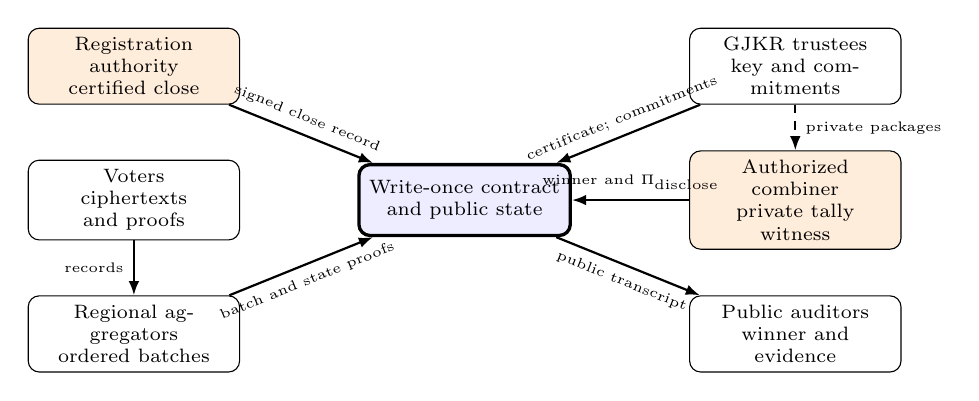
\begin{tikzpicture}[
  actor/.style={draw,rounded corners,align=center,text width=2.45cm,
                minimum height=9mm,font=\scriptsize},
  core/.style={actor,fill=blue!7,very thick},
  trust/.style={actor,fill=orange!14},
  pub/.style={-{Latex[length=1.8mm]},thick},
  priv/.style={-{Latex[length=1.8mm]},thick,dashed}
]
\node[core] (contract) at (0,0) {Write-once contract\\and public state};
\node[trust] (ra) at (-4.2,1.7) {Registration authority\\certified close};
\node[actor] (voter) at (-4.2,0) {Voters\\ciphertexts and proofs};
\node[actor] (agg) at (-4.2,-1.7) {Regional aggregators\\ordered batches};
\node[actor] (trustee) at (4.2,1.7) {GJKR trustees\\key and commitments};
\node[trust] (combiner) at (4.2,0) {Authorized combiner\\private tally witness};
\node[actor] (auditor) at (4.2,-1.7) {Public auditors\\winner and evidence};
\draw[pub] (ra) -- node[above,sloped,font=\tiny]{signed close record} (contract);
\draw[pub] (voter) -- node[left,font=\tiny]{records} (agg);
\draw[pub] (agg) -- node[below,sloped,font=\tiny]{batch and state proofs} (contract);
\draw[pub] (trustee) -- node[above,sloped,font=\tiny]{certificate; commitments} (contract);
\draw[priv] (trustee) -- node[right,font=\tiny]{private packages} (combiner);
\draw[pub] (combiner) -- node[above,font=\tiny]{winner and $\Pi_{\rm disclose}$} (contract);
\draw[pub] (contract) -- node[below,sloped,font=\tiny]{public transcript} (auditor);
\end{tikzpicture}
\caption{System architecture and trust boundaries.  Solid arrows are public
or contract-visible; the dashed arrow is the private authenticated delivery
of committed threshold packages.  Orange roles carry the explicitly stated
trust assumptions.}
\label{fig:architecture}
\end{figure}

The symbols $\mathsf{QUAL}$ and $S$ have different meanings:
$\mathsf{QUAL}$ is the GJKR dealer set that survives qualification, whereas
$S$ is the final set of $\tau$ trustees whose private packages are selected as
usable by the authorized combiner.  For $n\geq2t+1$, the protocol fixes
\[
 \tau=t+1,\qquad q_{\rm cert}=n-t.
\]
The first profile is $(n,t,\tau,q_{\rm cert})=(5,2,3,3)$,
with static corruption $|\mathcal C_T|\leq t<n/2$.  Privacy against direct
key reconstruction requires fewer than $\tau$ exposed shares.  Availability
requires at least $\tau$ distinct usable private packages actually delivered; malicious,
offline, invalid, and late trustees all consume the same total missing-share
budget $n-\tau=2$.

\subsection{Weighted ElGamal and group requirements}\label{subsec:bc-ind}
\label{subsec:semivoting-instantiation}

Let $\mathbb G_{\rm enc}=\langle g\rangle$ have prime order $q$.  The setup
record fixes
\[
 (\mathsf{groupID},q,g,\mathsf{encodingID},h_{\rm VSS},\mathsf{hashSuite}).
\]
Every group input has one canonical encoding and passes group and subgroup
checks.  The generator is nonidentity, no participant knows
$\log_g h_{\rm VSS}$, and the certified key satisfies
$PK_{\rm enc}\in\mathbb G_{\rm enc}\setminus\{1_{\mathbb G}\}$.  A valid
individual verification share $VK_h$ may equal the identity when the
corresponding Shamir share is zero; it is instead checked against the common
coefficient record.

For weighted one-hot value $m_{i,j}=v_{i,j}w_i$, encryption is
\[
 ct_{i,j}=(ct_{i,j}^0,ct_{i,j}^1)
 =(g^{r_{i,j}},PK_{\rm enc}^{r_{i,j}}g^{m_{i,j}}).
\]
Component-wise multiplication yields
\[
 CT_j=(g^{R_j},PK_{\rm enc}^{R_j}g^{M_j}),\qquad
 R_j=\sum_i r_{i,j},\quad M_j=\sum_i m_{i,j}.
\]
The allowed auxiliary information must preserve DDH in
$\mathbb G_{\rm enc}$.  In particular, a Type-3 pairing deployment must not
publish a cross-group element with the encryption-key exponent that enables a
pairing test of the small ballot message space.  Groth16's use of pairings does
not by itself make its source group suitable for ElGamal; an independent group
is permitted only with measured circuit and contract costs.

\begin{table}[htbp]
\centering
\caption{Cross-component compatibility obligations}
\label{tab:group-compatibility}
\small
\begin{tabular}{p{0.23\textwidth}p{0.64\textwidth}}
\toprule
Component & Required compatibility check \\
\midrule
ElGamal and GJKR & Same $\mathbb G_{\rm enc}$, order $q$, generator, subgroup rules, and canonical point encoding. \\
Chaum--Pedersen & Same encryption group and scalar field; the statement contains the frozen election and target identifiers. \\
Groth16 ballot circuit & Exact in-circuit representation and constraints for $PK_{\rm enc}$, ciphertext points, scalars, and public-input widths. \\
SnarkPack and state proof & Same audited ballot verification key, ordered public inputs, supported batch sizes, relation digests, and encoding map. \\
Contract and manifest & Native operations or verified wrappers for every selected group, field, hash, and pairing operation; byte-for-byte agreement with $\mathsf{PM}_e$. \\
\bottomrule
\end{tabular}
\end{table}

Table~\ref{tab:proof-relations} separates the four proof relations that are
sometimes conflated in an end-to-end description.  In particular,
$\Pi_{\rm valid}$ authenticates an ordered list of ballot statements but does
not prove the ciphertext transition; that role belongs to
$\Pi_{\rm state}$.

\begin{table}[htbp]
\centering
\caption{Proof relations and their public binding responsibilities}
\label{tab:proof-relations}
\small
\begin{tabular}{p{0.15\textwidth}p{0.31\textwidth}p{0.40\textwidth}}
\toprule
Relation & Principal public binding & Private witness or claim boundary \\
\midrule
$C_{\rm vote}$ & $eid$, $ctx_e$, certified key, closing root, nullifier, region, and ballot ciphertext & Credential, registered weight and opening, one-hot vote, and encryption randomness. \\
$\mathcal R_{\rm agg}^{(B)}$ & Exact ordered matrix of $B$ ballot public inputs under one audited $vk_{\rm vote}$ & Aggregates the corresponding Groth16 proofs; it does not establish a state update. \\
$C_{\rm state}^{(B)}$ & Batch identifier and root, $CT_{\rm old}$, $CT_{\rm new}$, context, and key digest & Ordered ballot records whose ciphertexts fold exactly from the old state to the new state. \\
$C_{\rm disclose}$ & Frozen target, registration and policy digests, selected commitments, and public winner & Share packages, commitment openings, CP transcripts, Lagrange reconstruction, and bounded tally.  Its nested-proof soundness is conditional. \\
\bottomrule
\end{tabular}
\end{table}

\subsection{Proof systems and auxiliary primitives}\label{sec2.2}

At the abstract level, a SNARK is a succinct non-interactive argument, and a
zk-SNARK additionally provides the required zero-knowledge property for the
instantiated relation.  In the concrete protocol, we use Groth16 as the
zk-SNARK for encrypted weighted-ballot validity and proved state transitions
\cite{bib32}.  We adopt SnarkPack to aggregate the resulting Groth16 ballot
proofs under one fixed verification key and compatible public-input layout
\cite{bib128}.  Separately, election key establishment instantiates the
distributed key-generation protocol of Gennaro, Jarecki, Krawczyk, and Rabin
(GJKR) \cite{bib133}.  These names identify concrete constructions and their
assumptions; they do not by themselves establish that the voting relations,
encodings, setup artifacts, or composition are sound.

\subsubsection{Groth16 and generalized Chaum--Pedersen}\label{subsec:nizk}
Groth16 proves the context-bound ballot relation and the batch state relation.
Computational soundness of the exact instantiated relations is used for
accepted-ballot and state correctness; no extractor is needed for those
claims.  By contrast, the winner-disclosure relation hides complete
Chaum--Pedersen transcripts inside an outer Groth16 witness.  Its intended
soundness argument therefore assumes an applicable knowledge-sound Groth16
interface that extracts those transcripts, partial shares, commitment
openings, and decoded tally---not any trustee's long-term secret share
\cite{bib32,bib34}.  Ordinary computational soundness of the outer proof does
not by itself expose an inner statement to which Chaum--Pedersen soundness can
be applied.  Knowledge soundness is also distinct from simulation
extractability; the latter is not assumed unless a later privacy proof names
and instantiates it.  The
stronger simulation interface needed by the privacy hybrids is separated as
proof obligation A3.  Generalized Chaum--Pedersen proves, for one trustee
witness $x_h$,
\[
 VK_h=g^{x_h}\quad\land\quad
 D_{h,j}=(CT_j^0)^{x_h}\quad\text{for every }j.
\]
Its statement includes the election, final context, trustee identifier,
verification share, frozen target, complete ciphertext vector, and complete
share vector.
The manifest defines $H_q:\{0,1\}^*\rightarrow\mathbb Z_q$ by a named
hash-to-field suite with rejection sampling and a fixed domain separator.  The
Fiat--Shamir soundness claim is in the classical random-oracle model and uses
an applicable generalized forking reduction \cite{bib132}; no standard-model or
quantum-random-oracle claim is made.  A concrete security report must include
the adversary's hash-query bound and the resulting forking loss.

\subsubsection{Joint proof, CRS, and hash model}
\label{subsec:joint-proof-model}
For the formal winner-disclosure protocol, the outer extractor and inner
Fiat--Shamir reduction must coexist in one explicitly defined experiment.  It
must specify CRS generation and auxiliary information, the adversary's access
to the outer prover and random oracle, the extraction order, rewinding or
forking compatibility, and the query bounds $Q_{\rm final}$ and $Q_{H'}$.
If the circuit implements a concrete hash, its byte encoding and bounded
hash-to-field algorithm must match the off-circuit verifier exactly.  If the
security proof instead idealizes that hash as a random oracle, the paper must
provide the corresponding circuit/ROM bridge.  This joint model and its exact
reduction are open obligations; Section~\ref{subsec:threshold-winner-disclosure} states
only the conditional interface they must satisfy.

\subsubsection{SnarkPack}\label{subsec:snarkpack}
For $B=2^\nu$ Groth16 proofs sharing one exact verification key and public-input
width, SnarkPack authenticates the complete ordered public-input matrix and
compresses the proof object and cryptographic verification core
\cite{bib128}.  Publication and processing of the $B$ public inputs remain
linear.  Residual ballots use binary decomposition into supported sizes, with
$B=1$ handled by direct Groth16 verification.

\subsubsection{PRFs, commitments, Merkle trees, and contracts}
\label{subsec:aux-blocks}
Election-scoped PRFs derive registration and ballot nullifiers.  A binding and
hiding commitment records the authorized weight; a Merkle proof binds it to an
approved registration root.  Domain-separated hashes commit to setup
manifests, key records, ordered batches, regional closing records, and the
unique tally target.  The contract is modeled as an append-only deterministic
state machine with atomic check-then-write operations.

These are parameterized primitives rather than implicit ``secure hash''
placeholders.  The proof manifest records one PRF family and its input/output
lengths, one commitment scheme with message/randomness spaces and binding and
hiding notions, one EUF--CMA signature scheme for trustee authentication, and
one hash suite with a domain/range entry for every use.  The correctness
theorems are conditional on those named notions.  A concrete deployment claim
requires actual scheme identifiers and parameters and adds their advantages,
hash-collision probabilities, proof-system soundness errors, and
Fiat--Shamir losses by a union bound.  Because this version provides no such
deployment manifest, it makes no concrete-bit-security claim.

\subsection{Threat, setup, and deployment assumptions}\label{sec2.3}
\label{subsec:trust-assumptions}

Trustee corruption is static before DKG.  GJKR uses authenticated confidential
channels, reliable broadcast, its specified timing and recovery rules, and an
authenticated roster.  The DKG agreement mechanism, certificate verifier, and
write-once registry are separate assumptions.  A certificate authenticates an
agreed public decision; it does not prove private-deal correctness by itself.

The formal winner-only settlement adopts the \emph{publicly tally-hiding} trust model:
the authorized combiner is trusted for confidentiality and inevitably learns
the full decoded tally before proving the winner.  It may be co-located with
the decoder and disclosure prover.  Its correctness is not trusted: the
contract accepts a winner only after verifying the exact disclosure relation.
Running several combiners may improve availability but does not reduce this
confidentiality trust boundary, because every authorized combiner that receives
$\tau$ usable packages learns the full tally.  Corruption of that combiner, compromise of
its private channel, or collusion in which it releases the decoded vector
reveals the tally and is outside Definition~\ref{def:th-function-equal}.  No
claim of fully tally-hiding computation, in which even internal authorities do
not learn the tally, is made.  Availability of the combiner is also an
explicit liveness assumption rather than a consequence of the trustee
threshold.

The RA is assumed honest for the certified aggregate: before signing it checks
eligibility, registration uniqueness, the authorized integer weight of every
canonical entry, and equality between each entry and its weight commitment,
then computes the exact integer sum.  Its signature authenticates this
assertion; it does not cryptographically prove that a dishonest signer computed
a hidden sum correctly.  This is a deliberate trust assumption of the current
profile, not a sum-SNARK claim.

Each trustee also has a registered authentication key
$(pk_h^{\rm auth},sk_h^{\rm auth})$.  In the privacy experiment the challenger
generates and retains every honest $sk_h^{\rm auth}$ and reproduces any
external-PKI certificate and validation record required by the deployment.
There is no unrestricted honest-signing oracle.  The experiment may invoke
$\mathsf{SimHonestAuth}$ only for an honest registered trustee, after
$H_{\rm target}$ is frozen, at the protocol-prescribed send point, at most once
for that trustee and target, and only on a message binding
$(eid,ctx_e,H_{\rm target},h_e^{\rm policy,pre},h_e^{\rm disclose},h,cm_h)$.
Corrupted trustees' commitments,
signatures, private packages, and scheduling actions are never replaced.

Groth16 and SnarkPack parameters are generated by the identified auditable
procedures.  The deterministic $\mathsf{VerifySetupArtifacts}$ algorithm checks
the exact relation digests, public-input widths, curves, encodings, verification
keys, supported batch sizes, and setup transcripts committed by
$\mathsf{PM}_e$.  Public ballot data must remain available.  The chain supplies
the stated ordering and finality semantics.  No theorem guarantees delivery of
trustee shares, decoding service, or settlement transactions.

\begin{definition}[Real disclosure success]
\label{def:th-real-success}
A real winner-disclosure execution succeeds only if an authorized combiner
obtains at least $\tau$ usable private share packages, decodes every tally
coordinate in its prescribed integer range, constructs an accepting disclosure
proof, and the corresponding settlement transaction becomes final.  Here a
package is usable exactly when delivery, commitment opening, and the complete
Chaum--Pedersen verification all succeed.
\end{definition}

\begin{definition}[Simulated public outcome]
\label{def:th-simulated-outcome}
$\mathsf{SimulatePublicOutcome}$ exists only inside a specified privacy hybrid.
It receives the allowed leakage, adversarial actions, and fixed delivery and
settlement schedule.  It need not execute bounded decryption on an intermediate
challenge ciphertext.  Its observable result, timing, and abort behavior must
be proved computationally indistinguishable from the corresponding real
endpoint distribution.  The real protocol never calls this algorithm.
\end{definition}

Thus real execution correctness, artificial-hybrid simulation capability, and
privacy between two real elections are three distinct claims.  In particular,
an accepting simulated proof is not evidence that an artificial transcript has
real-election semantics.

\section{Unified GJKR-DKG Voting Protocol}\label{sec3}

We adopt the GJKR distributed key-generation protocol as the foundation of
election key establishment.  Our election-specific certification layer does
not modify that DKG primitive; it additionally binds the agreed key to the
authenticated trustee roster, election parameters, verifier configuration,
and immutable protocol state.  The decryption threshold $\tau=t+1$ and the
certificate threshold $q_{\rm cert}=n-t$ serve different purposes and are
checked separately throughout the construction.

\subsection{Election context and certified key}\label{subsec:threat-upgrade}
\label{subsec:key-registration}

Before DKG, the election freezes the candidate and trustee rosters, parameters,
predicate, region assignment, proof manifest, registration policy and
authority key, tally rule, deadlines, and
$\mathsf{releasePolicyID}=\mathtt{WINNER\_ONLY\_V1}$ in a pre-key record
$P_e$.  The derived $kctx_e$ fixes both the pre-DKG policy digest and one DKG
session identifier.  Neither value depends on the post-DKG context $ctx_e$.
The sole key-establishment interface is
\[
 \mathsf{TDKG.Run},\quad\mathsf{TDKG.VerifyOutput},\quad
 \mathsf{TDKG.Finalize}.
\]
Section~\ref{subsec:threshold-dkg} specifies the GJKR messages and
qualification rules; Algorithm~\ref{alg:threshold-key-finalize} is the
normative finalizer.  Its accepted output is
\[
 \mathsf{CertifiedKey}_e=
 (K_e^{\rm core},h_e^{\rm key},ctx_e,Cert_e),
\]
where $K_e^{\rm core}$ contains the recovery-adjusted common coefficient
record, $PK_{\rm enc}=\overline A_0\neq1_{\mathbb G}$, every derived $VK_h$,
the trustee roster, threshold, $\mathsf{QUAL}$, and DKG transcript digest.
For compatibility with the ballot layout,
\[
 \mathsf{keySetHash}_e:=h_e^{\rm key}
\]
denotes only the certified DKG KeyCore digest; it is not a hash of candidate
keys.

Finalization accepts only if
\[
 \mathsf{DKGOutputAgreed}=1\ \land\
 \mathsf{CertificateValid}=1\ \land\
 \mathsf{RegistryWriteOnce}=1.
\]
If $PK_{\rm enc}=1_{\mathbb G}$, the session enters
$\mathsf{SETUP\_ABORT}$.  An authorized fresh session with new randomness and
a new identifier may begin only before voting; no accepted ballot is ever
re-keyed.

\subsection{Eligibility registration and certified closing record}
\label{subsec:registration-commitment}
For one canonical credential identifier $cid_i$, the RA enforces a global
election-scoped registration nullifier before authorizing one voter seed and
address.  Voter $i$ commits to the authorized nonnegative integer weight $w_i$
with opening $s_i$.  The RA checks eligibility, identifier uniqueness, the
weight-policy decision, and equality between the canonical entry and its
commitment before inserting that entry into the registration tree.

The setup fixes $W_{\max}<q$, one RA verification key, a registration-format
version $v_{\rm reg}$, one canonical rule identifier $\mathsf{ruleID}_e$, the
associated deterministic function $F_e$, and
$\mathsf{releasePolicyID}=\mathtt{WINNER\_ONLY\_V1}$.  These policy fields are
included in $P_e$.  Immediately after $P_e$ and $kctx_e$ are frozen, and
before the DKG session begins, the contract computes and stores
\[
\begin{aligned}
 h_e^{\rm policy,pre}=H(&\mathtt{VV/DISCLOSURE/POLICY/PRE/v2}\parallel\\
 &\mathsf{Encode}(eid,kctx_e,W_{\max},\mathsf{ruleID}_e,
                  \mathsf{releasePolicyID},
                  v_{\rm reg},pk_{\rm RA})).
\end{aligned}
\]
Registration close reuses this immutable value; it does not recompute a
nominally ``pre'' digest from the later $ctx_e$.
Let $\mathcal E_e$ be the canonical ordered set of accepted entries.  The RA
computes the integer sum and registry digest
\[
 W_{\rm registered}:=\sum_{i\in\mathcal E_e}w_i,qquad
 H_{\rm canonicalRegistry}:=H(\mathsf{Encode}(\mathcal E_e)),
\]
and forms
\[
\begin{split}
 \mathsf{RegClose}_e:=(&eid,ctx_e,RT_e^{\rm close},N_{\rm registered},
 W_{\rm registered},W_{\max},\\
 &h_e^{\rm policy,pre},v_{\rm reg},H_{\rm canonicalRegistry}),\\
 m_e^{\rm reg}:={}&H(\mathtt{VV/REGISTER/CLOSE/v1}\parallel
                  \mathsf{Encode}(\mathsf{RegClose}_e)),\\
 \sigma_e^{\rm reg}:={}&\mathsf{Sign}_{sk_{\rm RA}}(m_e^{\rm reg}),qquad
 \mathsf{Cert}_e^{\rm reg}:=(\mathsf{RegClose}_e,\sigma_e^{\rm reg}).
\end{split}
\]
Algorithm~\ref{alg:close-registration} verifies the signature, election and
context, canonical root and count, version, $0\leq W_{\rm registered}\leq
W_{\max}<q$, and equality with the immutable pre-policy fields.  Acceptance
freezes all closing fields and defines
\[
 h_e^{\rm disclose}:=H(\mathtt{VV/DISCLOSURE/CLOSE/v1}\parallel
             \mathsf{Encode}(\mathsf{Cert}_e^{\rm reg},
                             \mathsf{ruleID}_e)).
\]
The signature authenticates the RA's assertion; it does not prove that a
dishonest signer computed the hidden integer sum correctly.  Hence exactness
of $W_{\rm registered}$ relies on the stated RA-honesty assumption and is not
presented as a sum-SNARK result.

One accepted election-scoped nullifier permits at most one counted one-hot
ballot per certified entry.  RA-honest exact summation, valid committed ballot
weights, one-hot validity, and global nullifier uniqueness therefore give
\[
 0\leq M_j\leq W_{\rm registered}\leq W_{\max}<q,
\]
so each exponent has a unique bounded integer interpretation.  The function
$F_e(\vec M)$ returns the ordered set of maximal-score candidate identifiers;
a single-winner deployment selects the smallest canonical identifier.  This
tie rule is bound by $\mathsf{ruleID}_e$ and cannot be chosen by the combiner.

\subsection{Groth16 weighted ballot}\label{subsec:zk-voting}
Voter $i$ publishes
\[
 u_i=(eid,ctx_e,k,RT_i,nf_i,\mathsf{keySetHash}_e,
       PK_{{\rm enc},e},\vec{ct}_i)
\]
and proves with witness
$(vsk_i,addr_i,w_i,s_i,cm_i,\rho_i,\vec v_i,\vec r_i)$ that:
\begin{enumerate}
 \item $\vec v_i$ is a legal one-hot ballot;
 \item the PRF-derived address and deterministic region $k$ are correct;
 \item $nf_i$ is the election-scoped voting nullifier;
 \item $RT_i=RT_e^{\rm close}$ and the weight commitment is a member of that
       RA-certified canonical closing root; and
 \item every $ct_{i,j}$ is the weighted ElGamal encryption equation under the
       public $PK_{{\rm enc},e}$ contained in the certified registry record.
\end{enumerate}
The contract retrieves $(ctx_e,h_e^{\rm key},PK_{{\rm enc},e})$ from the
write-once registry and compares them with the proof instance.  It never
accepts a caller-supplied alternative verification key or election key.

\subsection{Batch settlement and threshold tally}\label{subsec:vv-dk-tally}
Section~\ref{sec5} defines $\mathsf{Groth16VoteVerify}$,
$\mathsf{SnarkPackVerify}$, $\mathsf{StateTransitionVerify}$, and the atomic
$\mathsf{SubmitBatch}$ transition.  Section~\ref{sec:threshold-mode} defines
the sole formal result-release procedure.  After
$\mathsf{FreezeTallyTarget}$, trustees publish authenticated commitments to
privately delivered share packages.  An authorized combiner validates a
usable private threshold and invokes
$\mathsf{BuildWinnerDisclosure}$ followed by the contract's
$\mathsf{AcceptWinnerDisclosure}$.  The contract accepts only the proof-backed
winner and never publishes the decoded vector or usable decryption shares.
Direct publication of a decoded tally is retained solely as an evaluation
baseline and is not a permitted terminal state of the formal election
protocol.

\begin{definition}[VeriVoting-Batch formal release protocol]\label{def:vv-security}
An accepted execution uses one certified nonidentity GJKR key, accepts only
ballots satisfying the five statements, applies each accepted ordered ballot
exactly once to regional state, and freezes one global tally target.  The
trusted combiner learns the bounded tally from at least $\tau$ usable private
packages, but the public transcript discloses only authenticated package
commitments, the deterministic outcome, and a proof for the frozen disclosure
relation.  Publication of the tally vector, partial-decryption shares, or
Chaum--Pedersen package proofs is not a valid release transition.
Its settlement soundness is conditional on Lemma~\ref{thm:th-disclosure-soundness}
and its undischarged joint-extraction premises.  Its public-view privacy target
is Definition~\ref{def:th-function-equal}; it is not a theorem of this paper
and is not claimed complete until A2, A3,
TH-AUTH, public-outcome simulation, and the full Function-Equal composition
are proved.
\end{definition}

\section{Security Claims and Proof Boundaries}\label{sec4}

The results are separated into five layers: T1 is certified GJKR key
consistency; T2 is exact ballot/batch accounting; T3 is registration
weight-bound consistency under RA honesty; T4 is a conditional nested
Chaum--Pedersen winner-settlement claim; and T5 is the Function-Equal privacy
definition, whose proof remains open.  In particular, T4 and T5 are not
promoted to unconditional theorems.  Table~\ref{tab:security-status} also maps
these layers to the four contributions and distinguishes a defined relation,
a conditional implication, an implemented check, and a complete composition
theorem.  Presence of one evidence type must not be read as evidence of the
others.

\begin{table}[htbp]
\centering
\caption{Security results, evidence, and current proof status}
\label{tab:security-status}
\small
\begin{tabular}{p{0.06\textwidth}p{0.11\textwidth}p{0.27\textwidth}p{0.42\textwidth}}
\toprule
Layer & Maps to & Result & Evidence and explicit boundary \\
\midrule
T1 & C1 & One immutable certified GJKR key and consistent verification shares & Defined finalization checks and conditional theorem (Theorem~\ref{thm:threshold-key-consistency}); assumes faithful GJKR, authenticated channels, reliable broadcast, certificate checking, and write-once finalization. \\
T2 & C2 & Accepted ballots are exactly the ordered records applied to the ciphertext state & Defined relations and conditional theorem (Theorem~\ref{thm:batch-security}); assumes sound Groth16, SnarkPack, and state relations, canonical encoding, collision resistance, and data availability.  End-to-end implementation evidence is evaluated separately. \\
T3 & C2/C4 & The registered integer bound uniquely constrains every tally coordinate & Proposition~\ref{prop:registration-weight-bound} under the explicit honest-RA aggregate assumption; no hidden-sum SNARK or complete malicious-RA theorem is claimed. \\
T4 & C3/C4 & A valid public winner is derived from the frozen target using committed private packages & Conditional lemma (Lemma~\ref{thm:th-disclosure-soundness}); fixed-profile native and frozen-storage fallback checks (Table~\ref{tab:prototype-verifiers}) are implemented. General circuit validation, the joint extraction argument, and exact SnarkPack EVM integration remain open. \\
T5 & C4 & Function-Equal public tally hiding & Formal definition and proof program only; external-key DKG simulation, proof-chain simulation, public-outcome simulation, and full composition remain open. \\
\bottomrule
\end{tabular}
\end{table}

\begin{proposition}[Proof-parameter consistency]
\label{prop:proof-key-consistency}
If $\mathsf{SetupConsistent}_e(\mathsf{PM}_e,\mathsf A_e)=1$, canonical
encodings and collision-resistant manifest hashes bind every installed
Groth16 and SnarkPack verifier to the exact published relation, public-input
width, curve, batch size, and $vk_{\rm vote}$.  A transaction cannot select a
different verifier after key finalization.
\end{proposition}

\begin{proposition}[DKG ballot-key binding]
\label{prop:vote-finalized-key}
Assume certified GJKR key consistency, Proposition~\ref{prop:proof-key-consistency},
Groth16 soundness, and the contract's equality checks.  If a ballot instance is
accepted, every proved ciphertext coordinate uses the same
$PK_e^{\rm DKG}=PK_{\rm registry}=PK_{\rm circuit}\neq1_{\mathbb G}$ fixed by
the election registry.
\end{proposition}

\textit{Justification.}  The ballot relation uses its public key input in every
ElGamal equation.  The verifier is fixed by the manifest, while the contract
compares the instance's context, KeyCore digest, and public key with write-once
storage.  A different key therefore requires proof-system failure, an explicit
equality-check failure, or a hash/encoding collision.

\begin{lemma}[State-to-certified-batch binding]
\label{lem:state-certified-batch}
Assume collision resistance of the domain-separated batch-tree hash,
canonical injective encoding of ballot records, SnarkPack soundness for the
listed Groth16 relations, and soundness of $C_{\rm state}^{(B)}$.  Except with
the sum of the corresponding failure probabilities, the ordered public-input
matrix verified by SnarkPack and the ballot records used by the state proof in
an accepted batch are the same sequence.  Consequently,
\[
 CT_{e,k,b}=CT_{e,k,b-1}\oplus
             \bigoplus_{i\in U_{k,b}}ct_i.
\]
The state circuit need not re-prove each encryption equation: that property is
supplied by the individual Groth16 relation and
Proposition~\ref{prop:vote-finalized-key}.
\end{lemma}

\textit{Justification.}  The contract recomputes the batch root from the
canonical ordered public records.  The state circuit exposes the same root and
recomputes it from its encoded record sequence.  Distinct sequences with the
same root yield either a non-injective record encoding or a collision in a
leaf or inner-node hash.  Conditioned on their equality, state-proof soundness
gives the displayed transition, while SnarkPack soundness supplies the listed
ballot-verification equations.

\begin{proposition}[Registration weight-bound consistency (T3)]
\label{prop:registration-weight-bound}
Assume RA honesty, EUF--CMA security of the registered RA signature scheme,
binding of the weight commitments, sound ballot relations, and global
election-scoped nullifier uniqueness.  If
$\mathsf{CloseRegistration}$ and all counted ballots are accepted, then every
decoded tally coordinate satisfies
\[
 0\leq M_j\leq W_{\rm registered}\leq W_{\max}<q.
\]
Except for the listed primitive failures, the values and registry root used at
settlement are the unique values authenticated by
$\mathsf{Cert}_e^{\rm reg}$.
\end{proposition}

\textit{Justification.}  Honest RA processing counts every canonical
registration exactly once and signs its exact integer sum.  Commitment binding
prevents a ballot from opening an entry to another weight, ballot soundness
gives a weighted one-hot contribution, and nullifier uniqueness prevents
reuse.  The contract freezes the signed closing record.  The proposition
would be false for a malicious RA that knowingly signs a wrong hidden sum;
signature verification alone cannot remove that assumption.

The established correctness chain is certified GJKR key consistency,
ballot-to-DKG-key binding, Groth16/SnarkPack/state soundness, exact encrypted
state, Chaum--Pedersen share validity, Lagrange reconstruction, and bounded
integer verification.  For winner-only disclosure, soundness additionally
uses binding share commitments, the exact compiled disclosure relation, the
winner rule, non-wrapping tally bounds, an applicable outer knowledge
extractor, and a compatible joint inner-proof reduction.  These last premises
remain open.  The separate privacy program is
L1 multi-message ElGamal IND-CPA, L2 external-key GJKR simulation, L3 audited
proof-chain simulation, L4 authenticated-commitment and public-outcome
simulation, and L5 full Function-Equal composition.  Only L1 is proved here;
the remaining interfaces are not inferred from correctness.

\section{Certified Batch Verification and State Update}\label{sec5}

\subsection{Design goal and regional state}\label{subsec:batch-goal}

Verifying one Groth16 proof and updating the encrypted tally per voter is a
throughput bottleneck even though each proof is succinct.  The certified batch
layer proves both that every listed ballot is valid under the one GJKR key and
that exactly those ordered ciphertexts produce the next encrypted state.  The
electorate is deterministically partitioned into $N$ constituencies. The
registration authority $\mathcal{RA}_k$ may also operate the batch aggregator
for constituency $k$, but its output is never trusted without proof. For the
explicit election identifier $eid$ and constituency $k\in[N]$, the rollup
contract $\mathcal{SC}^{\rm rollup}_k$ maintains
\[
 \mathsf{State}_{eid,k}=
 (\mathsf{next}_{eid,k},CT_{eid,k},\mathsf{UsedNF}_{eid,k},
  \mathsf{AcceptedRT}_{eid,k}).
\]
In the concrete instantiation, Groth16 proves each encrypted-ballot relation,
and SnarkPack establishes \emph{batch validity} by aggregating compatible
Groth16 proofs.  Neither operation establishes the separately submitted
ciphertext transition.  The relation for $\Pi_{\rm state}$ establishes
\emph{exact state transition} by constraining the old state, canonical batch,
and new state together.  The two proofs share authenticated batch data, but
retain different statements, witnesses, and verification keys.

Here $\mathsf{next}_{eid,k}$ is the next admissible regional batch identifier, $CT_{eid,k}$ is the current encrypted tally vector, $\mathsf{UsedNF}_{eid,k}$ is the spent-nullifier map, and $\mathsf{AcceptedRT}_{eid,k}$ contains exactly the RA-certified $RT_e^{\rm close}$ after $\mathsf{CloseRegistration}$; earlier working roots cannot authorize a counted ballot. Batch identifiers and ciphertext states are independent across regions:
\[
 CT_{eid,k,0}\longrightarrow CT_{eid,k,1}\longrightarrow\cdots
 \longrightarrow CT_{eid,k,m_k}.
\]
After voting closes and every regional state is frozen, $\mathcal{SC}_{\rm agg}$ computes
\[
 CT_{eid}^{\rm final}=\bigoplus_{k=1}^{N}CT_{eid,k,m_k},
\]
and the trustee threshold procedure of Section~\ref{sec:threshold-mode}
operates on $CT_{eid}^{\rm final}$. The case $N=1$ gives a single global
rollup.

This cross-region operation is defined only when every region uses the same immutable encryption key and candidate-coordinate order:
\[
 \forall k,\qquad PK_{{\rm enc},e,k}=PK_{{\rm enc},e},
 \qquad
 \mathsf{CandidateOrder}_{e,k}=\mathsf{CandidateOrder}_{e}.
\]
The contract records a canonical closing tuple
\[
 \mathsf{RegionClose}_{e,k}=
 (k,m_k,ctx_e,CT_{eid,k,m_k},d_{e,k}),
\]
where $d_{e,k}$ hashes the domain-separated canonical encoding of the preceding fields.  A state is eligible for global aggregation only after the target chain's stated finality condition holds and the closing record becomes immutable.  Multiplication of ciphertexts under different public keys, or of positions having different candidate semantics, is undefined and rejected rather than treated as homomorphic aggregation.  Section~\ref{subsec:threshold-target} binds the complete vector of closing records to the one decryptable target.

\subsection{Election setup and fixed circuits}\label{subsec:batch-setup}

The canonical election context $ctx_e$ from Section~\ref{subsec:threat-upgrade} is created only after $\mathsf{TDKG.Finalize}$ and commits to $\mathsf{keySetHash}_e$, $PK_{{\rm enc},e}$, the authenticated trustee roster, predicate, assignment rule, contract domain, proof-system parameters, and deadlines. Both $C_{\rm vote}$ and $C_{\rm state}^{(B)}$ reserve public-input slots for $eid$ and the finalized context and key fields; those values are not hard-coded into the circuits. Consequently, proof-key generation precedes publication of $kctx_e$ and the DKG session, while ballot proving follows certified key finalization. Batch processing instantiates the exact context-bound ballot circuit as
\[
 (pk_{\rm vote},vk_{\rm vote})\leftarrow
 \mathsf{Groth16.Setup}(C_{\rm vote}).
\]
For each aggregated size $B\in\mathcal{B}_{\rm agg}=\{2^\nu:1\leq\nu\leq L\}$, setup publishes aggregation parameters
\[
 (crs_{\rm agg}^{(B)},vk_{\rm agg}^{(B)})\leftarrow
 \mathsf{SP.Setup}(1^\lambda,\mathcal{R}_{\rm agg}^{(B)})
\]
and a fixed-size state circuit key pair
\[
 (pk_{\rm state}^{(B)},vk_{\rm state}^{(B)})\leftarrow
 \mathsf{Groth16.Setup}(C_{\rm state}^{(B)}).
\]
The formal release protocol must fix one parameterized disclosure circuit
$C_{\rm disclose}^{(\tau,C,\mathsf{suiteID})}$ and publishes
\[
 (pk_{\rm disclose},vk_{\rm disclose})\leftarrow
 \mathsf{Groth16.Setup}(C_{\rm disclose}^{(\tau,C,\mathsf{suiteID})}).
\]
Its manifest entry commits to the complete relation of
Section~\ref{subsec:disclosure-relation}, including the exact
Chaum--Pedersen transcript hash, commitment scheme, canonical cross-domain
encoding, group and scalar identifiers, Lagrange-index convention, integer
bounds, and winner/tie policy.
It also fixes a maximum number of rejection-sampling iterations and accounts
for the probability that hash-to-field fails within that bound; an unbounded
``repeat until accepted'' procedure is not a circuit.  Every comparison with
$W_{\rm registered}$ or $W_{\max}$ uses an explicit bit/range decomposition,
and every non-native $\mathbb F_q$ or group operation is represented by the
specified limb widths, carry constraints, range checks, and canonical
reduction rules.  The first circuit configurations to be evaluated are P3-A
$(5,2,3,C=3)$, P3-B $(7,3,4,C=3)$, P3-C $(9,4,5,C=3)$, and P3-D
$(7,3,4,C=5)$.  No configuration is claimed instantiated until its manifest,
R1CS digest, setup transcript, and measurements are published.
The notation makes the configured size explicit; it does not imply that the original SnarkPack API accepts these arguments literally. Adding $eid$, $\mathsf{keySetHash}_e$, and $PK_{{\rm enc},e}$ changes the ballot public-input layout, so the published Groth16 and SnarkPack parameters must be generated for this exact version of $C_{\rm vote}$. All ballot proofs in an aggregate use the same circuit, SRS, $vk_{\rm vote}$, and public-input width. Ballot and state proofs use different verification keys and are not aggregated together. Before $kctx_e$ is published, $\mathsf{PM}_e$ fixes the exact circuit/R1CS digests, public-input widths, verifier digests, and aggregation-parameter identifiers. The publicly audited predicate $\mathsf{SetupConsistent}_e$ from Section~\ref{subsec:key-registration} requires each aggregation verifier to refer to the same $vk_{\rm vote}$, $B$, and $q_{\rm vote}$ and each state verifier to refer to the corresponding $C_{\rm state}^{(B)}$ and $q_{\rm state}^{(B)}$.  It also binds $vk_{\rm disclose}$ to the exact $C_{\rm disclose}$ digest and public-input width. At finalization, the installed records must match that manifest before the contract stores them in the write-once $\mathsf{ElectionRegistry}[ctx_e]$. A ballot, batch, or disclosure transaction can never supply or select a verification key. A remaining number of ballots is decomposed into power-of-two batches, for example $13=8+4+1$; the $B=1$ residual follows the explicit direct-Groth16 branch in Algorithm~\ref{alg:submit-batch}, not SnarkPack or an unproved dummy-padding rule.

SnarkPack requires structured aggregation parameters. As described in the source construction, a new aggregation ceremony can be avoided only if two compatible and independently generated powers-of-tau transcripts over the same bilinear group are already available \cite{bib128}. The circuit-specific Groth16 setups remain necessary and must be generated by an auditable multiparty procedure under the trust assumptions of Section~\ref{subsec:trust-assumptions}.

\subsection{Context-bound ballots and off-chain pre-verification}\label{subsec:batch-ballots}

For regional mode, voter $i$ uses the same public ballot instance and witness defined in Section~\ref{subsec:zk-voting}:
\[
\begin{aligned}
 u_i&=(eid,ctx_e,k,RT_i,nf_i,\mathsf{keySetHash}_e,
       PK_{{\rm enc},e},\vec{ct}_i),\\
 \omega_i&=(vsk_i,addr_i,w_i,s_i,cm_i,\rho_i,\vec v_i,\vec r_i).
\end{aligned}
\]
In addition to Statements 1--5, their explicit formulation enforces $k=\mathsf{Assign}(ctx_e,addr_i)$ and uses the public $PK_{{\rm enc},e}$ in every component-wise encryption constraint. Consequently, each eligible address has one deterministic nullifier domain and one writable region. The registration protocol must also reject a second address for the same eligibility credential in election $e$; otherwise, a global nullifier registry would be required.

The voter first derives the canonical fixed-width field vector $\widehat u_i=\mathsf{Encode}_{\mathbb F}(u_i)$ and computes
\[
 \pi_i\leftarrow\mathsf{Groth16.Prove}(pk_{\rm vote},\widehat u_i,\omega_i)
\]
and sends $(u_i,\pi_i)$ to the regional aggregator rather than directly requesting on-chain Groth16 verification. Upon receipt, the aggregator runs
\[
 \mathsf{Groth16.Verify}(vk_{\rm vote},\widehat u_i,\pi_i).
\]
Invalid proofs are rejected before aggregation. This pre-verification only avoids wasted prover work when a candidate batch contains a bad proof; neither the contract nor the security argument trusts the result of this off-chain check.

\subsection{Canonical ordered batch}\label{subsec:batch-format}

Let the $b$-th batch in region $k$ be the ordered vector
\[
 U_{k,b}=(u_{k,b,0},\ldots,u_{k,b,B-1}).
\]
The canonical ordering defines an unambiguous representation of the accepted
ballot records for commitment, duplicate checks, replay protection, and
verification.  It is not required by the commutativity of homomorphic
ciphertext addition.  Two permutations therefore represent different batch
records even when their algebraic ciphertext product is equal.
Each structured instance is deterministically encoded as a fixed-width Groth16 field vector $\widehat u_i=\mathsf{Encode}_{\mathbb F}(u_i)$. Let $p_{\mathbb F}$ be the scalar-field modulus and $\ell_{\mathbb F}=\lfloor\log_2p_{\mathbb F}\rfloor-1$. The protocol first forms the canonical byte encoding in the displayed order
\[
\begin{aligned}
 (&eid,ctx_e,k,RT_i,nf_i,\mathsf{keySetHash}_e,
  \mathsf{Point}(PK_{{\rm enc},e}),\\
 &\mathsf{Point}(ct_{i,1}^0),\mathsf{Point}(ct_{i,1}^1),\ldots,
  \mathsf{Point}(ct_{i,|\mathcal C_e|}^1)).
\end{aligned}
\]
where $\mathsf{Point}(P)=(\mathsf{isInfinity},x(P),y(P))$ uses fixed-width big-endian coordinates and rejects noncanonical, off-curve, or wrong-subgroup points. Each fixed-width byte component is split into a protocol-fixed number of $\ell_{\mathbb F}$-bit big-endian limbs; every limb is range-constrained before injection into $\mathbb F$. Lengths are fixed by $\mathsf{PM}_e$, no leading zero may be dropped, and $\widehat u_i$ excludes the single leading constant that the Groth16 verifier itself prepends. The inverse decoding checks these ranges and reconstructs exactly the same bytes. Thus, the field vectors supplied to $\mathsf{SP.Verify}$ have exactly the same canonical content committed by the batch tree. Define
\[
\begin{aligned}
 L_i=H_{\rm leaf}(&\mathtt{VV/BATCH/LEAF/v2}\parallel eid\parallel ctx_e\parallel k
 \parallel b\parallel B\parallel i\\
 &\parallel |\widehat u_i|\parallel\mathsf{Encode}(\widehat u_i)).
\end{aligned}
\]
and use a separately domain-tagged inner-node hash to compute
\[
 R^{\rm batch}_{k,b}=\mathsf{MerkleRoot}(L_0,\ldots,L_{B-1}).
\]
We denote this complete leaf construction and domain-separated inner-node
computation by
$\mathsf{Root}_{v2}(eid,ctx_e,k,b,B,(\widehat u_i)_i)$; it is not a second
root function.
The index, length, and batch metadata make order and multiplicity unambiguous. Both the contract and $C_{\rm state}^{(B)}$ reject a record unless decoding and re-encoding it gives one unique canonical round trip; field reduction or an alternative group encoding is not accepted. The registration root $RT_i$ proves voter membership, whereas $R^{\rm batch}_{k,b}$ commits to the exact public ballot records, including their finalized key context, in this batch. The two roots have different domains and purposes. A voter need not know $b$ when producing $\pi_i$, because $b$ binds the later batch envelope, not the single-ballot relation.

\subsection{SnarkPack ballot-proof aggregation}\label{subsec:batch-validity}

For the fixed $vk_{\rm vote}$, the relation instantiated from SnarkPack is
\[
\begin{aligned}
 \mathcal{R}_{\rm agg}^{(B)}=\big\{&
  ((\widehat u_i)_{i=0}^{B-1},(\pi_i)_{i=0}^{B-1}):\\
 &\mathsf{Groth16.Verify}(vk_{\rm vote},\widehat u_i,\pi_i)=1
  \ \text{for all }i\in[0,B-1]\big\}.
\end{aligned}
\]
The aggregator generates
\[
 \Pi^{\rm valid}_{k,b}\leftarrow
 \mathsf{SP.Aggregate}\left(crs_{\rm agg}^{(B)},
 (\widehat u_i)_{i=0}^{B-1},(\pi_i)_{i=0}^{B-1}\right).
\]
SnarkPack commits to the vectors of Groth16 proof elements. Its Fiat--Shamir challenge binds the complete ordered public-input matrix and the proof-vector commitments, and its MT-IPP subargument proves the required random linear combinations of pairing and multiexponentiation equations \cite{bib128}. Verification therefore takes the full $(\widehat u_i)_{i=0}^{B-1}$, not only $R^{\rm batch}_{k,b}$. SnarkPack authenticates those complete public vectors through the Groth16 equations; it does not itself interpret their election semantics. Algorithm~\ref{alg:submit-batch} separately decodes each vector and compares $ctx_e$, $\mathsf{keySetHash}_e$, and $PK_{{\rm enc},e}$ with the immutable registry record.

Acceptance of $\Pi^{\rm valid}_{k,b}$ means that every listed individual Groth16 verification equation is valid under one $vk_{\rm vote}$. It does not prove that the listed ciphertexts were accumulated into $CT_{\rm new}$, nor that every ballot received by the aggregator was listed. These are separate state-consistency and liveness questions.

\subsection{Homomorphic batch transition and state proof}\label{subsec:batch-state}

Write the encrypted accumulator for candidate $j$ as $CT_j=(CT_j^0,CT_j^1)$ and ballot $i$ as $ct_{i,j}=(ct_{i,j}^0,ct_{i,j}^1)$. The aggregator reads the latest regional state $CT_{\rm old}=CT_{eid,k,b-1}$ and computes the component-wise group operation
\[
 CT_{{\rm new},j}^{h}=CT_{{\rm old},j}^{h}
 \prod_{i=0}^{B-1}ct_{i,j}^{h},
 \qquad j\in[|\mathbb C|],\ h\in\{0,1\}.
\]
This is the weighted-ElGamal homomorphism, applied once per batch instead of once per transaction.

Define the structured state statement and its fixed-width Groth16 field vector as
\[
\begin{aligned}
 x_{k,b}^{\rm state}&=(eid,ctx_e,k,b,B,R^{\rm batch}_{k,b},
 \mathsf{keySetHash}_e,PK_{{\rm enc},e},CT_{\rm old},CT_{\rm new}),\\
 \widehat x_{k,b}^{\rm state}&=
 \mathsf{Encode}_{\mathbb F}^{\rm state}(x_{k,b}^{\rm state}).
\end{aligned}
\]
The canonical byte string lists, in that displayed order, $eid$, $ctx_e$, $k$, $b$, $B$, $R^{\rm batch}_{k,b}$, $\mathsf{keySetHash}_e$, and $\mathsf{Point}(PK_{{\rm enc},e})$, followed first by $\mathsf{Point}(CT_{{\rm old},j}^{h})$ and then by $\mathsf{Point}(CT_{{\rm new},j}^{h})$ in lexicographic $(j,h)$ order. It uses the same fixed-width big-endian coordinates, limb decomposition, range constraints, no-truncation rule, and exclusion of Groth16's implicit leading constant as $\mathsf{Encode}_{\mathbb F}$. Every point must have one canonical on-curve prime-order-subgroup encoding. The identity is permitted for an accumulator component, including the initial encrypted zero, but not for $PK_{{\rm enc},e}$. Decoding followed by re-encoding must recover the same bytes. The manifest fixes
\[
 q_{\rm state}^{(B)}=|\widehat x_{k,b}^{\rm state}|.
\]

The public input of $C_{\rm state}^{(B)}$ is $\widehat x_{k,b}^{\rm state}$; its witness contains $U_{k,b}$ and the intermediate accumulators. The circuit (i) decodes the public vector and constrains its unique canonical round trip, (ii) canonically encodes every $u_i$ and checks its unique round trip, (iii) enforces for every record that its election identifier, context, region, key-set hash, and encryption key equal the corresponding public values, (iv) recomputes $R^{\rm batch}_{k,b}$, (v) extracts the ciphertext from each $u_i$, (vi) performs the group operation for both ciphertext components and every candidate, and (vii) constrains the final accumulator to equal $CT_{\rm new}$. The aggregator then generates
\[
 \Pi^{\rm state}_{k,b}\leftarrow
 \mathsf{Groth16.Prove}(pk_{\rm state}^{(B)},
 \widehat x_{k,b}^{\rm state},w_{k,b}^{\rm state}).
\]
If the encryption group is not native to the state circuit's scalar field, these group operations can dominate the constraint count. This cost is an implementation parameter to measure, not a free consequence of homomorphism.

\subsection{Atomic on-chain settlement}\label{subsec:batch-settlement}

The aggregator publishes the complete data-available transaction
\[
\begin{aligned}
 tx^{\rm batch}_{k,b}=(&eid,ctx_e,\mathsf{keySetHash}_e,PK_{{\rm enc},e},
 k,b,B,U_{k,b},R^{\rm batch}_{k,b},\\
 &CT_{\rm old},CT_{\rm new},\Pi^{\rm valid}_{k,b},
 \Pi^{\rm state}_{k,b}).
\end{aligned}
\]
Algorithm~\ref{alg:submit-batch} gives the settlement rule. For $B=1$, $\Pi^{\rm valid}_{k,b}$ denotes the original individual Groth16 ballot proof and $\Pi^{\rm state}_{k,b}=\bot$; the contract verifies that proof and performs the one-ballot ciphertext update directly. For $B\in\mathcal B_{\rm agg}$, the two batch proofs are required. All writes occur after all checks and are reverted together if any check fails.

\begin{algorithm}[H]
\caption{$\mathsf{SubmitBatch}(tx^{\rm batch}_{k,b})$}
\label{alg:submit-batch}
\begin{algorithmic}[1]
\Require $tx^{\rm batch}_{k,b}$ carrying $eid$ and regional state $\mathsf{State}_{eid,k}$
\State \textbf{require} $\mathsf{phase}[eid]=\mathsf{VOTING}$ and $\mathsf{keysFrozen}[eid]=\mathsf{true}$
\State \textbf{require} $ctx_e=\mathsf{currentContext}[eid]$
\State $K\gets\mathsf{ElectionRegistry}[ctx_e]$; \textbf{require} $K.\mathsf{status}=\mathsf{FINALIZED}$ and $K.eid=eid$
\State \textbf{require} $\mathsf{keySetHash}_e=K.\mathsf{keySetHash}$ and $PK_{{\rm enc},e}=K.PK_{\rm enc}$
\State \textbf{require} $b=\mathsf{next}_{eid,k}$, $(B=1\lor B\in\mathcal B_{\rm agg})$, and $|U_{k,b}|=B$
\State \textbf{require} $CT_{\rm old}=CT_{eid,k}$
\State \textbf{require} $\mathsf{CanonicalGroup}(K.PK_{\rm enc},CT_{\rm old},CT_{\rm new})$ with nonidentity $K.PK_{\rm enc}$
\For{$i=0$ to $B-1$}
  \State $\widehat u_i\gets\mathsf{Encode}_{\mathbb F}(u_i)$; \textbf{require} $\mathsf{CanonicalRoundTrip}(u_i,\widehat u_i)$
  \State \textbf{require} $|\widehat u_i|=K.q_{\rm vote}$, $u_i.eid=eid$, $u_i.ctx=ctx_e$, and $u_i.region=k$
  \State \textbf{require} $u_i.\mathsf{keySetHash}=K.\mathsf{keySetHash}$ and $u_i.PK_{\rm enc}=K.PK_{\rm enc}$
  \State \textbf{require} $\mathsf{AcceptedRT}_{eid,k}[u_i.RT]=\mathsf{true}$
  \State \textbf{require} $\mathsf{UsedNF}_{eid,k}[u_i.nf]=\mathsf{false}$
  \State \textbf{require} $u_i.nf$ is distinct within $U_{k,b}$
\EndFor
\State \textbf{require} $R^{\rm batch}_{k,b}=\mathsf{Root}_{v2}(eid,ctx_e,k,b,B,(\widehat u_i)_i)$
\If{$B=1$}
  \State \textbf{require} $\mathsf{Groth16.Verify}(K.vk_{\rm vote},\widehat u_0,\Pi^{\rm valid}_{k,b})=1$
  \State \textbf{require} $CT_{\rm new}=CT_{\rm old}\oplus\vec{ct}_0$ and $\Pi^{\rm state}_{k,b}=\bot$
\Else
  \State \textbf{require} $\mathsf{SP.Verify}(K.vk_{\rm agg}[B],(\widehat u_i)_i,\Pi^{\rm valid}_{k,b})=1$
  \State $x\gets(eid,ctx_e,k,b,B,R^{\rm batch}_{k,b},K.\mathsf{keySetHash},K.PK_{\rm enc},CT_{\rm old},CT_{\rm new})$
  \State $\widehat x\gets\mathsf{Encode}_{\mathbb F}^{\rm state}(x)$; \textbf{require} $|\widehat x|=K.q_{\rm state}[B]$ and $\mathsf{CanonicalRoundTrip}(x,\widehat x)$
  \State \textbf{require} $\mathsf{Groth16.Verify}(K.vk_{\rm state}[B],\widehat x,\Pi^{\rm state}_{k,b})=1$
\EndIf
\For{$i=0$ to $B-1$}
  \State $\mathsf{UsedNF}_{eid,k}[u_i.nf]\gets\mathsf{true}$
\EndFor
\State $CT_{eid,k}\gets CT_{\rm new}$; $\mathsf{BatchRoot}_{eid,k}[b]\gets R^{\rm batch}_{k,b}$
\State $\mathsf{next}_{eid,k}\gets b+1$
\end{algorithmic}
\end{algorithm}

The equality $CT_{\rm old}=CT_{eid,k}$ prevents a mathematically valid proof over a stale state from rolling the contract back. The explicit $eid$ namespace and regional sequence number prevent cross-election replay, repetition, and reordering. Checking every accepted registration root prevents an adversary from supplying an arbitrary root for which it knows a path. Nullifiers are checked both against prior batches and inside the current batch before being marked spent. The deterministic region assignment in $C_{\rm vote}$ prevents the same address from moving its nullifier to another regional map.

\subsection{Illustrative four-voter batch}\label{subsec:batch-example}

Consider candidates $A,B,C$ and four voters: Alice has weight $3$ and selects $A$; Bob has weight $2$ and selects $B$; Carol has weight $1$ and selects $A$; Dave has weight $4$ and selects $C$. Their hidden weighted vectors are $(3,0,0)$, $(0,2,0)$, $(1,0,0)$, and $(0,0,4)$. Each voter sends $(u_i,\pi_i)$ to the aggregator, which pre-verifies the four proofs and forms the ordered $B=4$ vector
\[
 U_{k,1}=(u_A,u_B,u_C,u_D).
\]
It canonically encodes these four records and computes
$R^{\rm batch}_{k,1}=\mathsf{Root}_{v2}
(eid,ctx_e,k,1,4,(\widehat u_i)_i)$ and
$\Pi^{\rm valid}_{k,1}$, then evaluates
\[
 CT_1=CT_0\oplus ct_A\oplus ct_B\oplus ct_C\oplus ct_D
\]
and proves this transition with $\Pi^{\rm state}_{k,1}$. The plaintext interpretation $(4,2,4)$ is used only to explain correctness; neither the aggregator transaction nor the contract reveals it before decryption. Once Algorithm~\ref{alg:submit-batch} accepts, $CT_{eid,k}$ changes atomically from $CT_0$ to $CT_1$ and all four nullifiers become spent. The next regional batch must use $CT_1$ as its old state.

\subsection{Security properties and limitations}\label{subsec:batch-security}

\begin{theorem}[Accepted-batch validity and exact accounting]\label{thm:batch-security}
Assume Proposition~\ref{prop:proof-key-consistency}, Theorem~\ref{thm:threshold-key-consistency}, and Proposition~\ref{prop:vote-finalized-key}. Thus $\mathsf{ElectionRegistry}[ctx_e]$ contains one immutable, certified nonidentity GJKR encryption-key record, and its audited verifier family has the exact circuit, width, and batch-size meanings committed by $\mathsf{PM}_e$. Assume computational soundness of Groth16 for $C_{\rm vote}$ and $C_{\rm state}^{(B)}$, SnarkPack soundness for $\mathcal{R}_{\rm agg}^{(B)}$ in the exact source-paper algebraic-group and random-oracle models, collision resistance of $H_{\rm key}$ and the context and batch hashes, binding of the voter commitment, and PRF security. Also assume that the eligibility layer maps each credential to one canonical identifier and atomically enforces the global $\mathsf{UsedRegNF}[eid]$ registry before any regional registration root is authorized. If Algorithm~\ref{alg:submit-batch} accepts $tx^{\rm batch}_{k,b}$ carrying $eid$, then, except with negligible probability: (i) every $u_i\in U_{k,b}$ belongs to the existential five-condition ballot relation under the unique finalized $PK_{{\rm enc},e}$; (ii) the exact ordered batch committed by $R^{\rm batch}_{k,b}$ satisfies
\[
 CT_{eid,k,b}=CT_{eid,k,b-1}\oplus
 \bigoplus_{i=0}^{B-1}\vec{ct}_i;
\]
and (iii) no accepted nullifier in this batch appeared in an earlier accepted batch of region $k$; moreover, (iv) one canonical eligibility credential cannot obtain a second registered address in another region.
\end{theorem}

\textit{Proof sketch.} The contract first checks the submitted $eid$, retrieves its final context, and obtains every verification key and public-input width from the immutable registry. Proposition~\ref{prop:proof-key-consistency} excludes a verifier for a different circuit, ballot key, width, or batch size, conditional on the stated setup audit. The contract also compares each canonically decoded record's election identifier, context, key-set hash, and encryption key with that registry. For $B>1$, SnarkPack soundness implies that every listed Groth16 verification relation holds; for $B=1$, the contract verifies the individual relation directly. Groth16 soundness implies that each accepted public instance belongs to the existential relation defined by $C_{\rm vote}$, and Proposition~\ref{prop:vote-finalized-key} binds every ciphertext equation to the finalized $PK_{{\rm enc},e}$. The contract computes the root from its public $U_{k,b}$, while $C_{\rm state}^{(B)}$ receives the uniquely encoded $\widehat x_{k,b}^{\rm state}$ and computes the same domain-separated root from its witness. Any different ordered vectors with the same root contradict collision resistance. State-proof soundness therefore gives the exact component-wise transition over those ciphertexts; the $B=1$ branch checks the transition directly. Equality with the current $CT_{eid,k}$ and the next regional identifier gives state continuity. The check-then-write ballot-nullifier rule gives regional uniqueness for one registered seed. Finally, deterministic region assignment prevents that seed from moving regions, while the globally atomic $rnf_i$ check prevents the same canonical eligibility credential from acquiring a second seed and address elsewhere.

For a fixed resource bound, write $\epsilon_{\rm key}$ for certified-key
failure, $\epsilon_{\rm SP}(B)$ for SnarkPack soundness, $\epsilon_{\rm G16}$
for one ballot proof, $\epsilon_{\rm state}(B)$ for the state proof,
$\epsilon_{\rm hash}(B)$ for all batch-tree and manifest collisions, and
$\epsilon_{\rm reg}$ for failure of the authenticated registration primitive.
A direct union bound gives
\[
 \epsilon_{\rm batch}(B)\leq \epsilon_{\rm key}
 +\epsilon_{\rm SP}(B)+B\epsilon_{\rm G16}
 +\epsilon_{\rm state}(B)+\epsilon_{\rm hash}(B)+\epsilon_{\rm reg}.
\]
This is an accounting identity, not a concrete security estimate: each term
must be instantiated at the same time, memory, and oracle-query bounds before
a bit-security claim is made.

Under its explicit global-registration assumption, the theorem establishes validity, validity-state consistency, state continuity, and duplicate-vote resistance for accepted public batches. Without that assumption, item~(iii) gives only regional nullifier uniqueness for a fixed registered seed. The theorem does not establish that every ballot delivered to an aggregator was included. Censorship resistance requires an authenticated intake log with deadlines, a forced-inclusion rule, or a direct-submission fallback. Likewise, a voter verifies inclusion by locating the canonical $u_i$ in an accepted, data-available $U_{k,b}$ and recomputing its batch root; a ciphertext-state change alone is not an individual receipt.

\subsection{Failure handling, data availability, and deployment}\label{subsec:batch-failures}

An invalid voter proof is discarded during pre-verification. If a submitted batch contains a spent or repeated nullifier, an unauthorized registration root, a bad canonical encoding, a stale $CT_{\rm old}$, a wrong sequence number, or a failed proof, the entire transaction reverts and the aggregator may rebuild a batch from the remaining records. This all-or-nothing rule prevents partial state updates.

The first version publishes $U_{k,b}$ as calldata or through a public data-availability layer with equivalent retrieval guarantees. Without the complete ordered inputs, the original SnarkPack verifier cannot reconstruct its Fiat--Shamir transcript, voters cannot check inclusion, and independent parties cannot reproduce the state transition. Consequently, proof size may be logarithmic while data publication, public-input folding, root computation, and nullifier storage remain $O(B)$.

Because $U_{k,b}$ is public, a contract with inexpensive native ciphertext operations could directly fold the batch and omit $\Pi^{\rm state}$. The state proof is useful only as verifiable outsourcing when direct group operations are more expensive than verifying the proof. Section~\ref{subsec:batch-evaluation} therefore includes a SnarkPack-only/direct-fold ablation.

The SnarkPack reference implementation uses BLS12--381 and operations in the pairing target group \cite{bib128}; it does not supply a Solidity verifier or Ethereum gas measurements. A deployment therefore requires a chain exposing all compatible operations, a dedicated precompile, or a succinct wrapper proof. Until such a verifier is implemented, this paper treats $\mathsf{SP.Verify}$ as the rollup contract's cryptographic interface and does not infer Ethereum gas savings from the native SnarkPack timings.

\subsection{Evaluation methodology for batch mode}\label{subsec:batch-evaluation}

This subsection separates completed native measurements from the full
comparative evaluation, which remains incomplete. G1-E uses one archived
32-ballot D5/W32 proof pool, one verification key and the same research SRS.
Each batch size has 30 timed rounds after excluded warmups: 150 batch records
on one machine and pool, not 150 independent elections. Setup and ballot
proving are outside these windows. The 45 separate memory processes measure
warmed operation phases, not setup/proving peak memory; no strong tail claim
is made from 30 rounds. Table~\ref{tab:native-batch-measured} reports medians.

\begin{table}[htbp]
\centering
\caption{G1-E fixed-pool native timings: 30 rounds per batch size.}
\label{tab:native-batch-measured}
\small
\begin{tabular}{rrrr}
\toprule
$B$ & Individual verify (ms) & Aggregate verify (ms) & Aggregation (ms) \\
\midrule
2 & 0.967 & 3.128 & 4.361 \\
4 & 1.901 & 4.092 & 8.782 \\
8 & 3.944 & 4.831 & 16.769 \\
16 & 7.135 & 5.523 & 30.857 \\
32 & 15.447 & 6.481 & 52.507 \\
\bottomrule
\end{tabular}
\end{table}

At $B=16,32$, aggregate verification is faster in this native campaign,
but aggregation adds computation and aggregate proofs are larger than the
individual-proof collections at these sizes. This is not evidence of lower
complete settlement cost or EVM gas. G2-E additionally verifies two
consecutive B4 transitions over the same suite: the second old state equals
the first new state, and all six final ciphertext coordinates equal an
independent fold of eight distinct ballots. Skip, replay and reset reject
without updates. G2-E is a functional sample, not a repeated full Direct Fold
receiver comparison. Sources and reproduction commands are fixed by the
archive in Section~\ref{subsec:threshold-evaluation}.

The remaining comparison operationalizes RQ1
by separating three effects: transaction
batching, proof aggregation, and outsourcing of the ciphertext transition.
The core comparison is per-ballot verification, aggregated verification with
direct folding, and aggregated verification with a state proof.  The two
additional rows in Table~\ref{tab:batch-baselines} isolate transaction batching
and the alternative Gro16.Agg backend.  The original implementation already
uses Groth16, so ``original VeriVoting'' and ``per-ballot Groth16'' are not
distinct baselines.

\begin{table}[htbp]
\centering
\caption{Required end-to-end batch baselines}
\label{tab:batch-baselines}
\begin{tabular}{|p{0.20\textwidth}|p{0.34\textwidth}|p{0.34\textwidth}|}
\hline
\textbf{Mode} & \textbf{Ballot verification} & \textbf{Ciphertext transition} \\ \hline
Legacy & One transaction and one Groth16 verification per ballot & Per-ballot contract update \\ \hline
Transaction-batch & One transaction with $B$ individual Groth16 verifications & Direct contract fold \\ \hline
SnarkPack-only & One $\Pi_{\rm valid}$ verification & Direct contract fold over public $U$ \\ \hline
Gro16.Agg-only & One transparently aggregated Groth16 verification & Direct contract fold over public $U$ \\ \hline
Proposed & $\Pi_{\rm valid}$ and $\Pi_{\rm state}$ verification & Proved outsourced transition \\ \hline
\end{tabular}
\end{table}

A completed comparative artifact should first retain $B\in\{2,4,8,16,32\}$; larger batches are not prerequisites for closing the current evidence gap. It must report the total electorate, region count, candidate count, Merkle depth, public field elements per ballot, circuit constraints, curve, hardware, software versions, repetitions, median, and appropriately supported tail statistics. Required off-chain batch metrics are ballot proving time, pre-verification time per ballot and batch, aggregation time for SnarkPack and a reimplemented Gro16.Agg baseline, ciphertext-folding time, state-proof time, proof sizes, peak memory, throughput, and end-to-end latency. On-chain or target-verifier metrics must separately report aggregate-proof verification, $\Pi_{\rm state}$ verification, public-input and data-availability cost, nullifier reads and writes, context checks, state writes, total batch cost, and amortized cost per accepted vote. The two aggregation systems must use the same curve, circuit, public-input width, batch contents, hardware, and compiler configuration; timings copied from their source papers are not a valid cross-system baseline.  The end-to-end batch accounting identity is
\[
\begin{aligned}
 C_{\rm batch}={}&C_{\rm SP.Verify}+C_{\rm State.Verify}
 +C_{\rm PublicInputs}\\
 &+C_{\rm Nullifier}+C_{\rm Storage}
 +C_{\rm ContextCheck}+C_{\rm BatchData}.
\end{aligned}
\]

The analytical scaling boundaries are: ballot proving is $O(C_{\rm vote})$; pre-verification reads $B$ proofs; homomorphic folding is $O(B|\mathcal C_e|)$; $C_{\rm state}^{(B)}$ contains $O(B|\mathcal C_e|)$ group-transition work plus $B$ leaf hashes; the SnarkPack proof and cryptographic verification core are $O(\log B)$; but its public-input processing is $O(Bq)$ and nullifier work is $O(B)$. Across $M$ accepted ballots, the system settles approximately $M/B$ batches while total public data and nullifier storage remain linear in $M$.

Finally, adversarial tests include a DKG identity or non-subgroup public key,
an inconsistent KeyCore digest, a ballot encrypted under a stale key, a
cross-election proof replay, a post-finalization replacement attempt, and a
batch carrying a foreign context. Batch-specific tests also replace or reorder
one $u_i$, alter $CT_{\rm new}$, reuse an intra- or inter-batch nullifier,
submit an unauthorized $RT_i$, replay a batch identifier, and prove from a
stale $CT_{\rm old}$. Each test must revert without changing any state.
One mandatory omission test supplies four valid records and their valid ballot
proofs while constructing the proposed transition from only the first, second,
and fourth ciphertexts.  Acceptance of the validity aggregate must not make
this inconsistent state transition acceptable.
SnarkPack reports a native verifier crossover near 32 proofs and a proof-size
crossover near 150 proofs in its own BLS12--381, 350-public-input environment
\cite{bib128}; these values are reference points, not VeriVoting-Batch results.
The break-even batch size must be measured again for the voting circuit and
target chain.

\section{Certified GJKR-DKG and Verifiable Winner-Only Settlement}
\label{sec:threshold-mode}

\subsection{Motivation and scope}
\label{subsec:threshold-scope}

This section gives the sole formal key-establishment and result-release protocol.
An independently authenticated trustee set $\mathcal T_e$ generates one
$\tau$-of-$n$ key with GJKR and later decrypts only the frozen global tally
target.  Candidates remain tally coordinates and never hold election-key
shares.  Weighted ElGamal, the five ballot conditions, Groth16, SnarkPack, the
ordered batch root, and the state-transition relation all use the one certified
GJKR context.

For $n\geq2t+1$, the protocol fixes $\tau=t+1$ and
$q_{\rm cert}=n-t$.  The first deployment profile is
\[
 (n,t,\tau,q_{\rm cert})=(5,2,3,3),
\]
where at most $t$ trustees are corrupted statically before DKG.  The DKG
follows the complete 2007 \emph{Journal of Cryptology} specification of the
Gennaro--Jarecki--Krawczyk--Rabin protocol (GJKR) for discrete-logarithm
groups, not a new protocol assembled from selected Feldman checks
\cite{bib133,bib134}.  It assumes authenticated confidential point-to-point channels,
the reliable broadcast and timing model required by GJKR, and an authenticated
trustee roster fixed before the session.  Formal settlement privately combines
authenticated packages and releases only a deterministic winner value plus a
disclosure proof.  A full-tally procedure is retained only as an analytical
and experimental comparator; it is not a second protocol mode or terminal
election state.
The security interface separates three claims.  \emph{Share validity} checks
that each trustee contribution is well formed and targets the frozen
ciphertext.  \emph{Threshold reconstruction} shows that a qualified set of
valid contributions recovers the bounded tally.  \emph{Public disclosure
soundness} additionally shows that the released winner follows from that same
reconstruction and the authorized outcome rule.  Success of an individual
share proof or of native threshold reconstruction does not by itself establish
the third claim.
An end-to-end public-view privacy theorem, adaptive post-election corruption, proactive
refresh, and everlasting privacy are not established by this version.

\subsection{Trustee, channel, and group model}
\label{subsec:threshold-model}

Let $\mathbb G_{\rm enc}=\langle g\rangle$ be a prime-order group of order
$q$.  GJKR additionally uses $h_{\rm VSS}\in\mathbb G_{\rm enc}$ such that no
participant knows $\log_g h_{\rm VSS}$; one trustee may not choose
$h_{\rm VSS}=g^a$ while retaining $a$.  The parameter-generation transcript,
group identifier, canonical point encoding, subgroup rules, GJKR protocol
version, and channel/broadcast suite are committed before DKG.

The verifier checks $q$ and the claimed security level, requires a nonidentity
generator $g$, validates canonical encodings and subgroup membership for every
commitment, ciphertext component, and proof commitment, and checks all scalar
ranges.  The final encryption key must satisfy
\[
 PK_{\rm enc}\in\mathbb G_{\rm enc}\setminus\{1_{\mathbb G}\}.
\]
This restriction is intentionally not imposed on each $VK_h$: a legitimate
Shamir evaluation may be zero, in which case $VK_h=1_{\mathbb G}$.  Such a
verification share remains acceptable only when it is derived from the same
agreed coefficient record as the public key.

If $\mathbb G_{\rm enc}$ is a source group $\mathbb G_1$ of a Type-3 pairing,
the complete public-parameter distribution must support DDH in
$\mathbb G_1$ (the XDH setting) \cite{bib135}.  All DKG and threshold-key
elements
\[
 PK_{\rm enc},\ VK_h,\ C_{i,\ell},\ A_{i,\ell}
 \in\mathbb G_{\rm enc}
\]
remain in that encryption group.  Setup, DKG, proof, and circuit artifacts must
not expose $g_2^x$, $g_2^{x_h}$, or any other cross-group value that permits a
pairing test for the same exponent used by $PK_{\rm enc}$ or a reconstructing
set of shares.  Indeed, if $PK_2=g_2^x$ were public, a guess $m'$ for
$C_1=PK_{\rm enc}^{r}g^m$ could be tested by
\[
 e(C_0,PK_2)\stackrel{?}{=}e(C_1g^{-m'},g_2).
\]
Because weighted ballot components have a small message space, this is a
direct plaintext test.  The DDH assumption used below is therefore stated
relative to the full allowed auxiliary information, not merely an isolated
four-tuple.  An independent non-pairing encryption group is also admissible,
but its non-native circuit and contract costs must then be measured.

Index $i$ denotes a DKG dealer, $h$ a receiving trustee, and $j$ a candidate
coordinate.  Trustee $T_h$ ultimately holds $x_h$ and publishes verification
share $VK_h$.  The set of non-disqualified dealers is $\mathsf{QUAL}$; the set
whose usable private packages are selected by the combiner is $S$.  These sets
need not be identical.

\subsection{Concrete GJKR distributed key generation}
\label{subsec:threshold-dkg}

\subsubsection{Pedersen-VSS generation}
Each dealer $T_i$ chooses independent degree-$t$ polynomials
\[
 f_i(X)=\sum_{\ell=0}^{t}a_{i,\ell}X^\ell,
 \qquad
 f_i'(X)=\sum_{\ell=0}^{t}b_{i,\ell}X^\ell
\]
over $\mathbb Z_q$ and reliably broadcasts
\[
 C_{i,\ell}=g^{a_{i,\ell}}h_{\rm VSS}^{b_{i,\ell}}
 \quad(0\leq\ell\leq t).
\]
It sends the authenticated private message
\[
 \mathsf{Deal}_{i\rightarrow h}=
 (\mathtt{VV/DKG/DEAL/v1},eid,sid_e^{\rm DKG},i,h,
   s_{i,h},s'_{i,h})
\]
with $s_{i,h}=f_i(h)$ and $s'_{i,h}=f_i'(h)$.  Trustee $T_h$ accepts this
deal only if its sender, receiver, session, round, scalar encodings, and
signature are valid and
\[
 g^{s_{i,h}}h_{\rm VSS}^{s'_{i,h}}
 =\prod_{\ell=0}^{t}C_{i,\ell}^{h^\ell}.
\]

\subsubsection{Complaints and one common qualified set}
A failed check causes $T_h$ to reliably broadcast a domain-separated,
session-bound $\mathsf{Complaint}(i,h)$.  Dealer $T_i$ answers by broadcasting
the disputed $(s_{i,h},s'_{i,h})$.  Exactly as in the GJKR Pedersen-VSS phase,
$T_i$ is disqualified if it receives more than $t$ complaints or if any
complaint response fails the displayed Pedersen equation.  Timeouts and
malformed or missing responses are handled by the selected reliable-broadcast
implementation according to the same protocol rule.  Since all qualification
decisions depend on authenticated reliable-broadcast data, every honest
trustee derives the same set $\mathsf{QUAL}$.  A deployment that produces
different honest views $\mathsf{QUAL}_h$ aborts; it must not form
$x_h=\sum_i s_{i,h}$ from inconsistent dealer sets.

\subsubsection{Public-key extraction}
Only after $\mathsf{QUAL}$ is fixed does every $T_i\in\mathsf{QUAL}$ reliably
broadcast
\[
 A_{i,\ell}=g^{a_{i,\ell}}\quad(0\leq\ell\leq t).
\]
Trustee $T_h$ checks
\[
 g^{s_{i,h}}=\prod_{\ell=0}^{t}A_{i,\ell}^{h^\ell}.
\]
If this check fails, it broadcasts the pair
$(s_{i,h},s'_{i,h})$ that satisfies the earlier Pedersen equation but fails
the Feldman equation.  One valid complaint invokes the GJKR reconstruction
phase for dealer $i$, recovering its committed degree-$t$ polynomial and
replacing the disputed public coefficient record by the recovered
$(A_{i,\ell})_{\ell=0}^{t}$.  Thus public-key extraction is not reduced to
checking only the product of constant terms.

After all required recovery steps, define
\[
 \overline A_\ell=\prod_{i\in\mathsf{QUAL}}A_{i,\ell},
 \qquad
 PK_{\rm enc}=\overline A_0,
\]
\[
 x_h=\sum_{i\in\mathsf{QUAL}}s_{i,h}\pmod q,
 \qquad
 VK_h=\prod_{\ell=0}^{t}\overline A_\ell^{h^\ell}=g^{x_h}.
\]
If $\overline A_0=1_{\mathbb G}$, output verification fails and the session
enters $\mathsf{SETUP\_ABORT}$; the value is never repaired by substituting an
arbitrary group element.  Before voting, an authorized policy may start a new
independent session with a fresh $sid_e^{\rm DKG}$ and new secret
contributions.  After voting starts, re-keying is forbidden.  For an unbiased
exponent this exceptional event has probability $1/q$; privacy experiments
use the allowed nonzero-key distribution or account for the corresponding
statistical difference.
The implementation follows that 2007 GJKR specification for reconstruction,
timeouts, and aborts; the equations above identify its outputs rather than
replace those subprotocols.

The threshold wrapper exposes the interfaces
\[
\begin{gathered}
 \mathsf{TDKG.Init},\ \mathsf{TDKG.CreateDeals},\\
 \mathsf{TDKG.VerifyDeals},\ \mathsf{TDKG.HandleComplaints},\\
 \mathsf{TDKG.DetermineQUAL},\ \mathsf{TDKG.ExtractPublicKey},\\
 \mathsf{TDKG.VerifyOutput},\ \mathsf{TDKG.Finalize}.
\end{gathered}
\]
The public transcript contains signed reliable-broadcast messages,
commitments, complaints, responses, recovery records, $\mathsf{QUAL}$, and
the final public coefficient record.  Trustee state additionally contains the
private authenticated deals and local verification state.  A digest of the
public transcript is publicly auditable, but it is not claimed to let an
outsider repeat checks that require private deals.

\begin{table}[htbp]
\centering
\caption{Threshold-DKG message classes}
\label{tab:dkg-messages}
\scriptsize
\begin{tabular}{p{0.18\textwidth}p{0.18\textwidth}p{0.50\textwidth}}
\toprule
Message & Transport & Mandatory signed content \\
\midrule
$\mathsf{VSSCommit}$ & reliable broadcast & tag, $eid$, $sid_e^{\rm DKG}$, round, dealer, $(C_{i,\ell})_\ell$ \\
$\mathsf{Deal}$ & confidential authenticated channel & tag, election/session, round, dealer, receiver, $s_{i,h},s'_{i,h}$ \\
$\mathsf{Complaint}$ & reliable broadcast & tag, election/session, round, dealer, complainant, deal digest and reason \\
$\mathsf{ComplaintResp}$ & reliable broadcast & tag, election/session, round, dealer, receiver, disputed shares \\
$\mathsf{QUALRecord}$ & reliable broadcast & tag, election/session, transcript prefix digest, deterministic $\mathsf{QUAL}$ \\
$\mathsf{ExponentCommit}$ & reliable broadcast & tag, election/session, dealer, $(A_{i,\ell})_\ell$ \\
$\mathsf{ExtractFail}$ & reliable broadcast & tag, election/session, dealer, receiver, shares witnessing Pedersen success and Feldman failure \\
$\mathsf{RecoveryRecord}$ & reliable broadcast & tag, election/session, dealer, recovered polynomial/public coefficients and supporting transcript \\
\bottomrule
\end{tabular}
\end{table}

\subsubsection{External-key simulation interface}
\label{subsec:extkey-dkg-interface}

The privacy reduction needs a stronger interface than ordinary agreement on a
fresh DKG output.  For a static corrupted trustee set $\mathcal C_T$, define
\[
 \mathsf{ExtKeySimDKG}(1^\lambda,PK,\mathcal C_T,sid_e^{\rm DKG})
\]
to be an interactive simulator given an externally fixed $PK\in\mathbb
G_{\rm enc}$ but not its discrete logarithm.  It must interact online with the
corrupted trustees and preserve their messages and random tapes.  Its output
must include their correctly distributed private views and a public transcript
containing consistent $\mathsf{Deal}$, $\mathsf{Complaint}$,
$\mathsf{ComplaintResp}$, $\mathsf{QUALRecord}$,
$\mathsf{ExponentCommit}$, recovery, and abort records.  Honest private shares
delivered to a corrupted receiver must be scalars consistent with the public
commitments.  Complaint responses may not require the simulator to reveal an
unknown scalar.  The final $\mathsf{QUAL}$, coefficient record, verification
shares, and public key must be mutually consistent and have public key exactly
$PK$.

The same interface must extend through certification.  Corrupted trustee
signatures remain adversarial messages.  Honest signatures may be generated
only by the challenger-managed keys of Section~\ref{subsec:trust-assumptions},
for the exact protocol-prescribed message and send point; the simulator has no
oracle for arbitrary messages.  Every DKG-finalization signature must refer to
the reliable-broadcast decision already produced in the simulated execution.
If the deployment uses an external PKI, A2 must additionally simulate its
certificate issuance and validation evidence and prove consistency with that
real authentication model.  The result must pass
$\mathsf{VerifyCertificate}(m_e^{\rm cert},Cert_e)$ and the write-once contract
checks.  Thus the certificate authenticates a simulated DKG output; it does
not independently prove that the GJKR execution is secure.

The following algebraic fact is useful but deliberately weaker than this
interface.  Let $|\mathcal C_T|=t$, let the simulator choose corrupted scalar
shares $(x_c)_{c\in\mathcal C_T}$, and put
$J=\{0\}\cup\mathcal C_T$.  With $L_a^J$ denoting the Lagrange basis on $J$,
define for every trustee index $h$
\[
 VK_h=PK^{L_0^J(h)}
       \prod_{c\in\mathcal C_T}(g^{x_c})^{L_c^J(h)}.
\]
These elements are evaluations in the exponent of one degree-at-most-$t$
polynomial whose value at zero is $\log_gPK$ and whose corrupted evaluations
are the chosen $x_c$.  Consequently, for every legal set $S$ of $t+1$
trustees,
\[
 \prod_{h\in S}VK_h^{\lambda_h^S}=PK.
\]
This proves public-share programmability without knowing $\log_gPK$; it does
\emph{not} generate consistent Pedersen deals, complaints, recovery messages,
or certificates.  Establishing that the concrete GJKR wrapper realizes
$\mathsf{ExtKeySimDKG}$ is therefore proof obligation A2.  Until it is
discharged, a privacy result using this interface is only an Ideal-DKG or
conditional result, not a consequence of the cited GJKR theorem alone.
Public-share interpolation therefore remains only an algebraic subroutine; it
cannot stand in for the private VSS, complaint, recovery, authentication, and
abort distribution required by the real malicious-GJKR view.

\subsection{Acyclic key finalization}
\label{subsec:threshold-finalization}

To prevent a key hash, context, and certificate from containing one another,
threshold finalization uses a one-way dependency chain.  Before DKG, freeze
\[
\begin{aligned}
 P_e=(&\mathsf{chainID},\mathsf{contractID},eid,\\
 &\mathsf{paramsHash}_e,\mathsf{proofManifestHash}_e,\\
 &\mathsf{candidateRosterHash}_e,\mathsf{trusteeRosterHash}_e,\\
 &\mathsf{dkgProtocolID},n,t,\tau,q_{\rm cert},\\
 &\mathsf{predicate}_e,\mathsf{assignment}_e,\mathsf{rootPolicy}_e,\\
 &W_{\max},v_{\rm reg},pk_{\rm RA},\\
 &\mathsf{ruleID}_e,\mathsf{releasePolicyID},\mathsf{deadlines}_e)
\end{aligned}
\]
and compute
\[
 kctx_e=H_{\rm ctx}(\mathtt{VV/PREKEY/v3}\parallel
                    \mathsf{Encode}(P_e)),
\]
\[
\begin{aligned}
 h_e^{\rm policy,pre}=H(&\mathtt{VV/DISCLOSURE/POLICY/PRE/v2}\parallel\\
 &\mathsf{Encode}(eid,kctx_e,W_{\max},\mathsf{ruleID}_e,
                  \mathsf{releasePolicyID},v_{\rm reg},pk_{\rm RA})).
\end{aligned}
\]
Both values are stored before the DKG phase begins.  The session identifier is
then computed as
\[
 sid_e^{\rm DKG}=H(\mathtt{VV/DKG/SESSION/v1}\parallel kctx_e).
\]
Every DKG message contains the latter value.

Once GJKR completes, form the certificate-free record
\[
\begin{aligned}
 K_e^{\rm core}=(&eid,kctx_e,sid_e^{\rm DKG},\mathtt{THRESHOLD},
 \mathsf{dkgProtocolID},n,t,\tau,q_{\rm cert},\mathsf{QUAL},\\
 &PK_{\rm enc},(VK_h)_{h\in\mathcal T_e},H_{\rm DKG}),
\end{aligned}
\]
where $H_{\rm DKG}$ commits to the canonical public transcript and all
recovery-adjusted public coefficients.  Next compute
\[
 h_e^{\rm key}=H_{\rm key}(\mathtt{VV/KEYCORE/v3}\parallel
                           \mathsf{Encode}(K_e^{\rm core})),
\]
\[
 ctx_e=H_{\rm ctx}(\mathtt{VV/FINALCONTEXT/v3}\parallel
                   \mathsf{Encode}(kctx_e,h_e^{\rm key})).
\]
The message certified by authenticated trustee identity keys is
\[
 m_e^{\rm cert}=H(\mathtt{VV/DKG/FINALIZE/v1}\parallel
  \mathsf{Encode}(eid,sid_e^{\rm DKG},h_e^{\rm key},ctx_e)).
\]
The certificate $Cert_e$ contains signatures by at least
$q_{\rm cert}=n-t$ distinct
members of the frozen trustee roster, their identifiers, the certification
suite identifier, and the reliable-broadcast decision/transcript digest to
which those signatures refer.  An honest trustee signs at most one output and
only after deriving the common GJKR decision.  The contract checks roster
membership, the $q_{\rm cert}$ threshold, signature validity, the decision digest,
transcript and field equality, and then performs one write-once transition.  A
$3$-of-$5$ signature count alone is not treated as a non-forking proof: two
such signer sets may intersect only in corrupted trustees.  Agreement instead
uses reliable-broadcast agreement (which makes all honest signers certify the
same output) together with deterministic contract finalization.  If the
deployed certification layer cannot establish that link, it is an explicit
external consensus/audit premise.

The frozen record is
\[
 \mathsf{TK}_e^{\rm final}=
 (K_e^{\rm core},h_e^{\rm key},ctx_e,Cert_e),
\]
and the dependency graph is exactly
\[
\begin{aligned}
 P_e&\longrightarrow kctx_e
 \longrightarrow\{h_e^{\rm policy,pre},sid_e^{\rm DKG}\},\\
 sid_e^{\rm DKG}&\longrightarrow K_e^{\rm core}
 \longrightarrow h_e^{\rm key}\longrightarrow ctx_e
 \longrightarrow Cert_e.
\end{aligned}
\]
No object contains a digest or certificate computed downstream from itself.
The ballot slot is assigned
\[
 \mathsf{keySetHash}_e:=h_e^{\rm key},
\]
and denotes the certified DKG KeyCore rather than any candidate-key list.

Final acceptance separates three predicates.  First,
$\mathsf{DKGOutputAgreed}$ requires every completing honest trustee to use one
recovery-adjusted coefficient record and to derive
$PK_{\rm enc}=\overline A_0$ and
$VK_h=\prod_{\ell=0}^t\overline A_\ell^{h^\ell}$.  Second,
$\mathsf{CertificateValid}$ verifies distinct authorized identities,
signatures, the common election/session and KeyCore digest, and equality with
the reliable-broadcast decision.  Third, $\mathsf{RegistryWriteOnce}$ forbids
replacement of an accepted election record.  None of these predicates is
silently substituted for another: signatures alone do not prove the private
GJKR execution, and write-once storage alone does not repair a forked off-chain
decision.  Algorithm~\ref{alg:threshold-key-finalize} is the single normative
finalization procedure.

\begin{theorem}[Certified GJKR key consistency]
\label{thm:threshold-key-consistency}
Assume a faithful execution of the cited 2007 GJKR protocol with static
$t<n/2$ corruption, its authenticated private channels and reliable broadcast,
unknown $\log_g h_{\rm VSS}$, canonical encodings and collision-resistant
hashes, unforgeable trustee identity signatures, correct certificate-policy
checking, the explicit nonidentity-key check, and the write-once registry
transition.  If $\mathsf{DKGOutputAgreed}$,
$\mathsf{CertificateValid}$, and $\mathsf{RegistryWriteOnce}$ all accept, then
the election context binds one recovery-adjusted coefficient record; all
honest trustees agree on one $\mathsf{QUAL}$, one
$PK_{\rm enc}=g^{f(0)}\neq1_{\mathbb G}$, and verification shares
$VK_h=g^{f(h)}$ for one degree-$t$ polynomial $f$.  The accepted $ctx_e$
identifies one immutable $K_e^{\rm core}$ and certificate, except with the
failure probability of the stated primitives and DKG assumptions.
\end{theorem}

\textit{Justification.} GJKR correctness gives a common qualified set and
consistent shares after its prescribed complaint and recovery phases
\cite{bib133}.  Multiplication of the recovery-adjusted coefficient
commitments yields $\overline A_\ell=g^{f_\ell}$, hence
$PK_{\rm enc}=\overline A_0=g^{f(0)}$ and
$VK_h=\prod_\ell\overline A_\ell^{h^\ell}=g^{f(h)}$.  The acyclic digests,
nonidentity check, signature checks, and one-write registry bind that output to one election
record.  The theorem is conditional on the real broadcast/certification
implementation satisfying these interfaces; a hash by itself does not prove
that private deals were checked.

\subsection{Compatibility with certified ballot and batch verification}
\label{subsec:threshold-compatibility}

The ballot relation remains
\[
 ct_{i,j}^{0}=g^{r_{i,j}},\qquad
 ct_{i,j}^{1}=PK_{\rm enc}^{r_{i,j}}g^{v_{i,j}w_i}.
\]
Before accepting an individual ballot or batch, the contract checks
\[
 \mathsf{VerifyDKGFinalization}(\mathsf{TK}_e^{\rm final})=1,
\]
retrieves rather than accepts $PK_{\rm enc}$ and $h_e^{\rm key}$ from the
immutable registry, and requires every public instance to contain exactly
those values.  SnarkPack authenticates the complete ordered public-input
matrix, while the state proof binds the same records to
$CT_{\rm old}\rightarrow CT_{\rm new}$.

This is an interface-level reuse claim, not a claim that existing setup files
are automatically reusable.  The artifact audit must establish that
$PK_{\rm enc}$ is a true public input used by every encryption constraint, no
witness key can replace it, the positions and canonical encodings of
$(ctx_e,h_e^{\rm key},PK_{\rm enc})$ are unchanged, and the vote,
aggregation, and state verification keys correspond to those exact relations.
Any R1CS, curve, encoding, or width change requires new parameters and a new
manifest audit.

For privacy proofs we distinguish the real setup audit from the following
joint, reduction-only interface:
\[
 (\mathsf A_e,td_{\rm vote},td_{\rm state},td_{\rm disclose})
 \leftarrow\mathsf{JointSetupAndAudit}(1^\lambda,\mathsf{PM}_e).
\]
The public artifact bundle $\mathsf A_e$ must be indistinguishable from a real
accepted bundle and must pass the unchanged
$\mathsf{VerifySetupArtifacts}$ procedure for the exact circuits, public-input
widths, curve and encoding identifiers, verifier keys, and aggregation records
in $\mathsf{PM}_e$.  A component trapdoor is provided only when that component
actually requires proof simulation; no trapdoor is part of a protocol view.
For a random-DDH ballot instance with no known witness,
$td_{\rm vote}$ must produce an accepting proof for that exact instance.

The reduction otherwise uses real algorithms whenever it can compute the
witness.  In particular, accepting simulated Groth16 ballot proofs are fed to
the real $\mathsf{SP.Aggregate}$ algorithm as efficient postprocessing, rather
than to a newly assumed batch simulator, only after the following
\emph{TH-SPCompat} audit: every simulated proof verifies under the audited
ballot key; the real aggregator consumes exactly the ordered proof and
public-input vectors fixed by the batch transcript; its aggregate verifies
under the audited SnarkPack parameters; and neither aggregation nor
verification exposes a setup trapdoor.  This does not require reproving the
TIPP/MIPP construction, but it does require a concrete compatibility test for
the deployed artifacts.

The state-circuit audit likewise determines whether simulation is necessary.
If its witness consists only of public-computable ordered ciphertexts, Merkle
paths, indices, intermediate roots and canonical encodings, the reduction
runs the real state prover on the recomputed hybrid state.  If the compiled
circuit additionally requires voter secrets or encryption randomness, the
manifest must declare that fact and $td_{\rm state}$ must supply the exact
arbitrary-instance simulation interface.  The disclosure proof is simulated
only in hybrids where its private shares or decoded tally are unavailable or
do not exist; otherwise the real prover is used.  Ordinary Groth16 zero
knowledge does not by itself establish these joint setup, arbitrary-instance,
simulation-soundness, or artifact-compatibility properties.  Their verification
for the actual circuits and setup files is proof obligation A3/TH-CHAIN.

\begin{theorem}[Certified ballot and batch validity under GJKR-DKG]
\label{thm:threshold-certified-batch}
Under Theorem~\ref{thm:threshold-key-consistency},
Proposition~\ref{prop:proof-key-consistency}, the assumptions of
Theorem~\ref{thm:batch-security}, and the circuit-level public-key audit just
stated, every individual ballot or batch accepted by the protocol satisfies
the five ballot conditions under the unique DKG-generated
$PK_{{\rm enc},e}$; an accepted batch applies exactly those ordered
ciphertexts to the prior regional state.
\end{theorem}

\textit{Proof sketch.} Finalization supplies one immutable key record.
Canonical decoding and explicit contract equality checks bind each public
instance to that record.  Groth16 and SnarkPack soundness supply the ballot
relations, and the ordered root plus state-proof soundness supplies the exact
homomorphic transition, exactly as in Theorem~\ref{thm:batch-security}.

\subsection{Global closing records and the unique tally target}
\label{subsec:threshold-target}

Every required region must use the same finalized $PK_{{\rm enc},e}$,
$h_e^{\rm key}$, candidate count, candidate-coordinate order, and ciphertext
encoding.  The contract first requires one accepted and immutable
$\mathsf{Cert}_e^{\rm reg}$ and defines
\[
 H_{\rm RegClose}=H(\mathtt{VV/REGISTER/CLOSE/RECORD/v1}\parallel
                    \mathsf{Encode}(\mathsf{RegClose}_e)).
\]
Once all required $\mathsf{RegionClose}_{e,k}$ records from
Section~\ref{subsec:batch-goal} are final, order them by region identifier and
compute
\[
 H_{\rm close}=H(\mathtt{VV/REGION/CLOSESET/v1}\parallel
  \mathsf{Encode}((\mathsf{RegionClose}_{e,k})_{k=1}^{N})).
\]
The global contract then computes
\[
 CT_e^{\rm final}=\bigoplus_{k=1}^{N}CT_{eid,k,m_k}
\]
and freezes
\[
\begin{aligned}
 H_{\rm target}=H(&\mathtt{VV/TALLY/TARGET/v1}\parallel\\
 &\mathsf{Encode}(eid,ctx_e,h_e^{\rm key},h_e^{\rm policy,pre},\\
 &\qquad h_e^{\rm disclose},H_{\rm RegClose},H_{\rm close},
                  CT_e^{\rm final})).
\end{aligned}
\]
Closing the last required regional submission path moves the state from
$\mathsf{VOTING}$ to $\mathsf{REGIONS\_CLOSED}$; the subsequent target write
moves it to $\mathsf{TALLY\_TARGET\_FROZEN}$ and is irreversible.  No trustee share for
an individual ballot, adversarial ciphertext, stale regional state, different
coordinate order, or different election is accepted.

\subsection{Verifiable threshold partial decryption}
\label{subsec:threshold-partdec}

Trustee $T_h$ holding $x_h=f(h)$ computes for each candidate coordinate
\[
 D_{h,j}=(CT_j^0)^{x_h}.
\]
The generalized Chaum--Pedersen relation is stated with group equations so
that the boundary case $CT_j^0=1_{\mathbb G}$ is well defined:
\[
\begin{aligned}
 \mathcal R_{\rm dec}^{\rm th}=\{((&eid,H_{\rm target},ctx_e,h,
 VK_h,\vec{CT}^{\,0},\vec D_h),x_h):\\
 &VK_h=g^{x_h}\ \land\
 \forall j,\ D_{h,j}=(CT_j^0)^{x_h}\}.
\end{aligned}
\]
With fresh $\eta_h\leftarrow_R\mathbb Z_q$, the prover sets
\[
 A_{h,0}=g^{\eta_h},\qquad A_{h,j}=(CT_j^0)^{\eta_h},
\]
\[
\begin{aligned}
 d_h=H_q(&\mathtt{VV/THRESHOLD/DKEY/v1}\parallel\\
 &\mathsf{Encode}(eid,H_{\rm target},ctx_e,h,VK_h,
 \vec{CT}^{\,0},\vec D_h,A_{h,0},(A_{h,j})_j)),\\
 z_h&=\eta_h+d_hx_h\pmod q.
\end{aligned}
\]
The verifier reads every statement field from, or compares it with, the frozen
registry and tally target; validates canonical subgroup encodings and vector
lengths; and checks
\[
 g^{z_h}=A_{h,0}VK_h^{d_h},\qquad
 (CT_j^0)^{z_h}=A_{h,j}D_{h,j}^{d_h}\quad\forall j.
\]
The scalar $d_h$ is always recomputed from these bytes; it is neither accepted
as a caller-supplied value nor exposed as an unconstrained witness in P3.  A
P3 instantiation must implement the same manifest-pinned hash-to-field
algorithm and its bounded rejection branch.  Applying inner proof soundness
to transcripts extracted from P3 is subject to the joint model of
Section~\ref{subsec:joint-proof-model}, not to an independent black-box union
bound.
In the formal protocol, $(\vec D_h,\pi_h^{\rm dec})$ is placed inside the
private package $P_h$ rather than published or stored on chain.  The authorized
combiner performs the exact native verification before selecting a package,
and $C_{\rm disclose}$ verifies the same relation inside the final proof.  The
contract receives only the authenticated commitment described below.  A
public-share verifier is used solely by the full-tally evaluation baseline.

\subsection{Private threshold combination and bounded decoding}
\label{subsec:threshold-combination}

For $(n,\tau)=(5,3)$, $n-\tau=2$ is the total missing-share budget.  A
trustee that is maliciously silent, offline, late, or rejected for an invalid
private package all has the same availability effect.  Thus two unavailable
or rejected trustees can be tolerated when the other three deliver usable
packages, but two withholding trustees plus one additional offline honest
trustee cannot.  The static privacy bound $|\mathcal C_T|\leq2$ is not an
extra availability allowance, and a threshold number of public commitments
does not establish delivery of a usable private quorum.

The authorized combiner locks $S$ to the first $\tau$ usable packages under
the protocol's canonical receipt-order rule.  The adversary may influence
message scheduling and hence which valid set arrives first, but later packages
cannot change $S$.  For $h\in S$, compute
\[
 \lambda_h^S=\prod_{\substack{\ell\in S\\\ell\neq h}}
              \frac{-\ell}{h-\ell}\pmod q,
 \qquad
 D_j=\prod_{h\in S}D_{h,j}^{\lambda_h^S}.
\]
Then
\[
 Y_j=CT_j^1/D_j=g^{M_j}.
\]

The election parameters fix a public capacity $W_{\max}<q$, and registration
close freezes the tighter bound $W_{\rm registered}\leq W_{\max}$.  Therefore
\[
 0\leq M_j\leq W_{\rm registered}\leq W_{\max}<q
\]
for every coordinate and enforce compatible voter-count and weight bounds in
registration and the ballot relation.  The combiner may recover
$\widehat M_j=\log_gY_j$ by baby-step--giant-step or a precomputed bounded
table; the inequality gives uniqueness but not by itself efficiency.  The
disclosure relation accepts the private integer only if
\[
 0\leq\widehat M_j\leq W_{\rm registered}
 \quad\text{and}\quad
 g^{\widehat M_j}=Y_j
\]
for every $j$.  Only after all checks does
$\mathsf{WinnerCorrect}$ derive the public result $y=F_e(\vec M)$.  Neither
$Y_j$ nor $\widehat M_j$ is published by the formal protocol.

\begin{theorem}[Threshold-combination correctness]
\label{thm:threshold-tally}
Assume Theorem~\ref{thm:threshold-key-consistency}, soundness of the
generalized Chaum--Pedersen proof for $\mathcal R_{\rm dec}^{\rm th}$,
canonical subgroup checks, an immutable $H_{\rm target}$, and the bound
$0\leq M_j\leq W_{\rm registered}\leq W_{\max}<q$.  For every accepted set $S$ of $\tau=t+1$
distinct trustees, the algorithm above outputs the same
$Y_j=g^{M_j}$.  Every integer vector satisfying the bounded-decode checks is
the unique weighted tally in the declared range.  In the formal protocol this
vector is a private witness of the disclosure relation, not a public output.
\end{theorem}

\textit{Proof.} The accepted proof binds
$D_{h,j}=(CT_j^0)^{f(h)}$.  Lagrange interpolation at zero gives
$\sum_{h\in S}\lambda_h^Sf(h)=f(0)$, and hence
\[
 D_j=(CT_j^0)^{f(0)}.
\]
For $CT_j^1=PK_{\rm enc}^{R_j}g^{M_j}$ and
$CT_j^0=g^{R_j}$, division cancels
$(CT_j^0)^{f(0)}=PK_{\rm enc}^{R_j}$.  Finally, exponentiation by a generator
of order $q$ is injective on the declared interval of length less than $q$.

For comparison only, an evaluation harness may publish valid shares, apply the
same interpolation and exponentiation checks, and record the decoded vector.
This full-tally baseline measures threshold arithmetic and decoding costs; it
is not an executable result-release branch and contributes no public event to
the formal election state machine.  Appendix~A.2 gives its explicitly labeled
comparator algorithms.

\begin{theorem}[Conditional winner-only completion]
\label{thm:threshold-completion}
Suppose DKG and key finalization complete, every regional closing record and
the global tally target become final, and at least $\tau$ trustees publish
authenticated commitments and privately deliver usable packages before the
deadline.  Suppose additionally that the authorized combiner is available,
recovers the unique vector in
$[0,W_{\rm registered}]^{|\mathcal C_e|}$, generates an accepting disclosure
proof for $y=F_e(\vec M)$, and the chain finalizes the corresponding
$\mathsf{AcceptWinnerDisclosure}$ transaction.  Then the formal state machine
reaches $\mathsf{RESULT\_DISCLOSED}$ despite up to $n-\tau$ unavailable or
rejected trustees.  Malformed, duplicate, or undelivered packages and an
incorrect decoded vector cannot alter the accepted result, conditional on
Lemma~\ref{thm:th-disclosure-soundness}.  The theorem makes no termination
claim if a usable private quorum is absent, the combiner or decoder is
unavailable, proof generation fails, the settlement transaction is not
delivered, or finality fails.
\end{theorem}

This theorem is a conditional state-machine completion statement, not an
unconditional network-liveness, robustness, or unconditional P3-soundness
theorem: it assumes every event needed to enter the terminal state and the
named proof premise, and isolates only the effect of up to two unavailable or
rejected trustees in the first profile.

\subsection{Private share commitments and winner-only disclosure}
\label{subsec:threshold-winner-disclosure}

Winner-only disclosure is the unique formal settlement procedure of
VeriVoting-Batch.  After the certified final ciphertext is frozen, trustees
publish hiding commitments and authentication signatures while delivering
their complete partial-decryption packages over private authenticated
channels.  The contract never publishes individual decryption shares,
reconstructed group tally coordinates, or the decoded tally.  The full-tally
construction above is used only as an analytical and experimental comparator.
For
trustee $T_h$, define the private package
\[
 P_h=(eid,ctx_e,h_e^{\rm policy,pre},h_e^{\rm disclose},
       H_{\rm target},h,VK_h,CT_e^{\rm final},
       \vec D_h,\pi_h^{\rm dec})
\]
and publish
\[
 cm_h=\mathsf{Com}(\mathsf{Encode}(P_h);\rho_h),\qquad
 \sigma_h=\mathsf{Sign}_{sk_h^{\rm auth}}(m_h^{\rm com}),
\]
where
\[
 m_h^{\rm com}=H(\mathtt{VV/TH/COMMIT/v1}\parallel
 \mathsf{Encode}(eid,ctx_e,H_{\rm target},h,
                 h_e^{\rm policy,pre},h_e^{\rm disclose},cm_h)).
\]
Only $(h,cm_h,\sigma_h)$ is public.  The trustee sends
$(P_h,\rho_h)$ over the prescribed private authenticated channel to an
authorized combiner.  The public signature authenticates the commitment; it
does not certify that the committed package opens correctly or contains a
valid Chaum--Pedersen proof.  Corrupted trustees retain their real keys and
choose their own messages, omissions, and timings.

For a frozen target, let
\[
\begin{aligned}
 \mathsf{Delivered}_h&:=\text{the combiner receives }(P_h,\rho_h),\\
 \mathsf{CommitOpenValid}_h&:=
   [cm_h=\mathsf{Com}(\mathsf{Encode}(P_h);\rho_h)],\\
 \mathsf{CPValid}_h&:=
   [\mathsf{CPVerifyExact}(P_h)=1],\\
 \mathsf{Usable}_h&:=\mathsf{Delivered}_h\land
   \mathsf{CommitOpenValid}_h\land\mathsf{CPValid}_h,\\
 \mathsf{QuorumValid}&:=\left[\sum_{h\in\mathcal T_e}
                         \mathsf{Usable}_h\geq\tau\right].
\end{aligned}
\]
Here $\mathsf{CPVerifyExact}$ recomputes the Fiat--Shamir challenge from the
complete transcript in Section~\ref{subsec:threshold-partdec}; the challenge
is not a free circuit witness.  A commitment threshold therefore does not
imply a usable private quorum.

The unique success path of the formal election state machine is shown in
Figure~\ref{fig:winner-state-machine}.  Setup and voting must first traverse
$\mathsf{DKG\_RUNNING}\rightarrow\mathsf{KEY\_FINALIZED}
\rightarrow\mathsf{REGISTRATION}\rightarrow\mathsf{VOTING}
\rightarrow\mathsf{REGIONS\_CLOSED}$; the figure expands the subsequent
winner-only release path.

\begin{figure}[htbp]
\centering
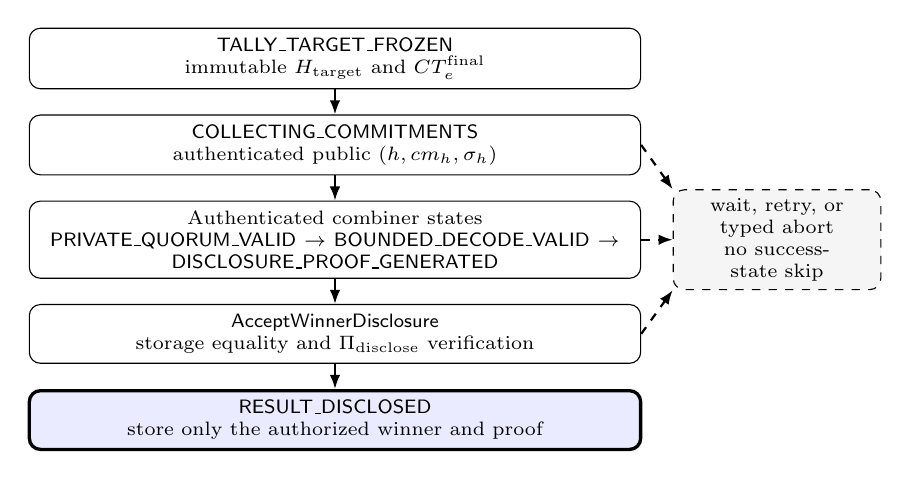
\begin{tikzpicture}[
  node distance=3.2mm,
  state/.style={draw,rounded corners,align=center,text width=.62\linewidth,
                inner sep=3.5pt,font=\scriptsize},
  terminal/.style={state,fill=blue!8,very thick},
  fail/.style={draw,dashed,rounded corners,align=center,text width=.20\linewidth,
               inner sep=3pt,font=\scriptsize,fill=gray!8},
  flow/.style={-{Latex[length=1.8mm]},thick}
]
\node[state] (target) {$\mathsf{TALLY\_TARGET\_FROZEN}$\\
  immutable $H_{\rm target}$ and $CT_e^{\rm final}$};
\node[state,below=of target] (commit) {$\mathsf{COLLECTING\_COMMITMENTS}$\\
  authenticated public $(h,cm_h,\sigma_h)$};
\node[state,below=of commit] (private) {Authenticated combiner states\\
  $\mathsf{PRIVATE\_QUORUM\_VALID}\rightarrow
   \mathsf{BOUNDED\_DECODE\_VALID}\rightarrow
   \mathsf{DISCLOSURE\_PROOF\_GENERATED}$};
\node[state,below=of private] (verify) {$\mathsf{AcceptWinnerDisclosure}$\\
  storage equality and $\Pi_{\rm disclose}$ verification};
\node[terminal,below=of verify] (result) {$\mathsf{RESULT\_DISCLOSED}$\\
  store only the authorized winner and proof};
\node[fail,right=4mm of private] (failure) {wait, retry, or typed abort\\
  no success-state skip};
\draw[flow] (target) -- (commit);
\draw[flow] (commit) -- (private);
\draw[flow] (private) -- (verify);
\draw[flow] (verify) -- (result);
\draw[flow,dashed] (commit.east) -- (failure.north west);
\draw[flow,dashed] (private.east) -- (failure.west);
\draw[flow,dashed] (verify.east) -- (failure.south west);
\end{tikzpicture}
\caption{Winner-only settlement state machine.  Invalid, missing, late, or
unfinalized inputs cannot transition to $\mathsf{RESULT\_DISCLOSED}$.}
\label{fig:winner-state-machine}
\end{figure}
The intermediate quorum, decode, and proof-generation states are authenticated
combiner states whose evidence is checked by the final disclosure relation;
the on-chain phase moves directly from commitment collection to
$\mathsf{RESULT\_DISCLOSED}$ only after proof verification.  Merely observing
$\tau$ public commitments never establishes
$\mathsf{PRIVATE\_QUORUM\_VALID}$.
An invalid opening, invalid decryption proof, unavailable combiner or decoder,
timeout, failed proof generation, rejected settlement transaction, or failed
finality predicate follows an explicit wait, retry, or typed-abort branch; it
does not skip to a later success state.  For the locked canonical set $S$ of
the first $\tau$ usable packages, define
\[
\begin{aligned}
 \mathsf{DecodeOK}&:=
   [\forall j:\ 0\leq M_j\leq W_{\rm registered}\ \land\ Y_j=g^{M_j}],\\
 \mathsf{FinalizeOK}&:=
   \mathsf{ProofValid}\land\mathsf{SettlementFinalized},\\
 \mathsf{RealSuccess}&:=
   \mathsf{QuorumValid}\land\mathsf{DecodeOK}\land\mathsf{FinalizeOK}.
\end{aligned}
\]

We write $\mathsf{ExecuteRealTH}$ for this executable protocol: it receives
real packages, verifies them, interpolates, bounded-decodes, computes
$y=F_e(\vec M)$, proves the disclosure relation, and waits for final settlement.
By contrast,
$\mathsf{ExecuteHybridTH}(\mathsf{FrozenPublicState},y^*,
\mathsf{OutcomeSchedule})$ is a proof-only experiment that may replace public
objects by simulated ones under a schedule fixed before the challenge.
$\mathsf{RealOutcome}$ is the actual result or typed abort of the former;
$\mathsf{SimulatePublicOutcome}$ is restricted to the latter and may emit only
the predetermined public result, proof, commitment, and timing/abort class.
It never invokes bounded decoding on a random-DDH ciphertext.  A simulated
transcript is not an alternative implementation of the protocol.

\subsection{Disclosure relation and conditional soundness}
\label{subsec:disclosure-relation}

For a manifest-pinned suite, the exact parameterized circuit
$C_{\rm disclose}^{(\tau,C,\mathsf{suiteID})}$ has public input
\[
\begin{aligned}
 x=(&eid,ctx_e,h_e^{\rm policy,pre},h_e^{\rm disclose},RT_e^{\rm close},
      W_{\rm registered},W_{\max},H_{\rm target},\\
    &CT_e^{\rm final},PK_{\rm enc},S,(VK_h,cm_h)_{h\in S},
      \mathsf{ruleID}_e,y)
\end{aligned}
\]
and witness
\[
 w=((\vec D_h,\pi_h^{\rm dec},\rho_h)_{h\in S},\vec M).
\]
$W_{\rm registered}$ is a run-time public input authenticated at registration
close; it is neither a secret witness nor a DKG-time circuit constant.
Its exact relation $\mathcal R_{\rm disclose}$ accepts if and only if all of
the following hold:
\[
\boxed{\begin{aligned}
 &\mathsf{InputPolicyRegistryBinding}\land\mathsf{CommitOpen}\\
 &{}\land\mathsf{CPVerifyExact}\land\mathsf{GroupMembership}\\
 &{}\land\mathsf{CanonicalEncoding}\land\mathsf{ExactLegalSet}\\
 &{}\land\mathsf{LagrangeCorrect}\land\mathsf{BoundedTallyCorrect}\\
 &{}\land\mathsf{WinnerCorrect}.
\end{aligned}}
\]
$\mathsf{InputPolicyRegistryBinding}$ checks every public field against the
frozen key, registration-close certificate, policy, root, target, ciphertext,
and disclosure manifest; it recomputes all relevant digests, including the
target binding to $\mathsf{RegClose}_e$ and $h_e^{\rm disclose}$.
$\mathsf{CommitOpen}$ reconstructs every $P_h$ and its commitment.
$\mathsf{CPVerifyExact}$ parses the complete transcript, recomputes
$d_h$ from the exact domain-separated canonical byte string with the fixed
bounded hash-to-field algorithm, and checks every generalized
Chaum--Pedersen equation.  In particular, $d_h$ is not an unconstrained
witness.
$\mathsf{GroupMembership}$ rejects the identity where prohibited and checks
the prime-order subgroup for every group element.
$\mathsf{CanonicalEncoding}$ uses one manifest-pinned conversion between
contract bytes, group elements, and circuit field limbs, rejecting aliases.
$\mathsf{ExactLegalSet}$ checks $|S|=\tau$, strict canonical ordering, distinct
nonzero indices, membership in the frozen trustee roster, and exact alignment
of every $(VK_h,cm_h)$ and private package.
$\mathsf{LagrangeCorrect}$ recomputes every coefficient in $\mathbb Z_q$ from
those indices and combines the shares.
$\mathsf{BoundedTallyCorrect}$ checks
$Y_j=CT_j^1/\prod_{h\in S}D_{h,j}^{\lambda_h^S}=g^{M_j}$ and
$0\leq M_j\leq W_{\rm registered}\leq W_{\max}<q$ for all $C$ coordinates,
using explicit integer bit/range decompositions and the manifest's non-native
field/group constraints.
$\mathsf{WinnerCorrect}$ checks $y=F_e(\vec M)$ using the public
$\mathsf{ruleID}_e$ and its fixed tie branch.  No election, policy, registry,
target, key, set, range, transcript-challenge, or result field may occur only
as an unconstrained witness value.

Before invoking $vk_{\rm disclose}$, the contract separately verifies each
$\sigma_h$ against the registered $pk_h^{\rm auth}$ and the exact message
containing $h_e^{\rm policy,pre}$, $h_e^{\rm disclose}$, and $cm_h$; the
circuit does not silently replace this outer authentication check.

The non-wrap premise follows from registration and ballot validity:
\[
 W_{\rm registered}=\sum_{i\in\mathcal E_e}w_i\leq W_{\max}<q,
 \qquad 0\leq M_j\leq W_{\rm registered}.
\]
One accepted nullifier per credential and the one-hot weighted ballot relation
ensure that no accepted credential contributes its weight twice or to two
coordinates.  Thus an exponent in the declared interval denotes one integer,
not merely a residue modulo $q$.

\begin{lemma}[Conditional nested CP verification soundness (T4)]
\label{thm:th-disclosure-soundness}
Assume T1--T3, one immutable target, unforgeable trustee authentication,
binding commitments, correct group/field compilation and canonical encoding,
and the non-wrap bound.  Assume further (i) an applicable knowledge-soundness
extractor for the exact outer Groth16 circuit that, from each accepted proof,
extracts the committed packages, complete Chaum--Pedersen transcripts,
openings, shares, and tally; and (ii) a joint experiment in which the inner
Fiat--Shamir reduction remains sound for those extracted transcripts under the
same CRS, auxiliary information, oracle programming, and extraction schedule.
Then, except with the parameterized failure bound below, contract acceptance
implies $y=F_e(\vec M_{\rm true})$ for the unique tally encrypted in
$CT_e^{\rm final}$.  The extractor is not required or asserted to recover any
trustee's long-term $x_h$.
\end{lemma}

\textit{Conditional argument.}  The assumed outer knowledge extractor exposes
a satisfying P3 witness rather than merely asserting that some witness exists.
Commitment binding and authentication attach the extracted packages to the
frozen public statement.  Only within the assumed joint experiment may inner
Chaum--Pedersen soundness then bind every extracted $\vec D_h$ to $VK_h$ and
the frozen ciphertext.  Lagrange combination reconstructs the certified
secret-key action, the range/non-wrap constraints select the unique integer
tally, and the winner circuit forces $y=F_e(\vec M)$.  Ordinary Groth16
computational soundness is insufficient for the first step, and knowledge
soundness does not automatically provide the simulation extractability needed
by a privacy hybrid.  The restricted compiled P3 prototype reported in
Section~\ref{subsec:threshold-evaluation} checks the implemented relation but
does not supply the assumed joint reduction or a general circuit audit.
This lemma therefore remains conditional.

For at most $Q_{\rm final}$ settlement attempts and $Q_{H'}$ relevant inner
hash queries, the intended accounting interface is
\[
\begin{aligned}
 \epsilon_{\rm GJKR}+\epsilon_{\rm batch}+\epsilon_{\rm reg}
 +\epsilon_{\rm auth}+\epsilon_{\rm bind}
 +\epsilon_{\rm KS}(Q_{\rm final})
 +\epsilon_{\rm CP}^{\rm joint}(\tau,Q_{\rm final},Q_{H'})\\
 {}+\epsilon_{\rm encoding}+\epsilon_{\rm policy}.
\end{aligned}
\]
Here $\epsilon_{\rm KS}$ is the applicable outer knowledge-soundness loss and
$\epsilon_{\rm CP}^{\rm joint}$ includes the exact extraction/forking and
bounded hash-to-field losses.  We do not identify the latter with
$Q_{\rm final}\tau\epsilon_{\rm CP}^{\rm single}$: such a product bound must
be derived, not presumed, for the concrete joint model.

\subsection{Threshold privacy games and proof boundary}
\label{subsec:threshold-privacy}

Let the adversary choose before DKG a static corrupted trustee set
$\mathcal C_T\subseteq\mathcal T_e$ with
$|\mathcal C_T|\leq t<\tau$.  It controls those trustees' random tapes,
messages, complaints, persistent states, signatures, and decision to withhold;
it receives their private states and the complete public transcript.  The
challenger, not the adversary, generates and retains every honest trustee
authentication secret key.  There is no general honest signing oracle.
The adversary does not corrupt the authorized combiner, decoder, or their
private delivery channels.  This exclusion is definitional rather than a
derived guarantee: any such corruption reveals the full tally reconstructed
by $\mathsf{ExecuteRealTH}$ and wins immediately.  The game therefore captures
only publicly tally-hiding confidentiality against observers, voters, and up
to $t$ corrupted trustees.

The experiment is selective.  Before any challenge ciphertext is released,
the adversary fixes the corrupted-voter ciphertexts and randomness, accepted
positions, regions, candidate-coordinate order, batch partition, final
inclusion set, frozen target rule, and a \emph{successful outcome schedule}.
The schedule names at least $\tau$ honest trustees that deliver valid private
packages before the deadline, an available combiner and bounded decoder, an
available disclosure prover, and a settlement transaction that satisfies the
configured confirmation rule.  It also fixes the canonical accepted set and
public timing class.  The game samples only from executions satisfying this
predeclared schedule; it does not run an arbitrary execution and condition
afterward on the event that it happened to succeed.  Adaptive corrupted-voter
submissions, challenge-dependent censorship, and failure-pattern privacy are
outside this first target.

The permitted public leakage is the typed tuple
\[
 \mathcal L_e=(\mathcal L_{\rm setup},\mathcal L_{\rm registry},
 \mathcal L_{\rm voting},\mathcal L_{\rm settlement},y).
\]
$\mathcal L_{\rm setup}$ contains public parameters, rosters, circuit and
suite identifiers, deadlines, and public DKG/certification metadata;
$\mathcal L_{\rm registry}$ contains $RT_e^{\rm close}$,
$N_{\rm registered}$, $W_{\rm registered}$, $W_{\max}$, registration-format
and policy identifiers, and the public closing certificate;
$\mathcal L_{\rm voting}$ contains corrupted voters and trustees, accepted
positions, regions, batch sizes and partitions, inclusion metadata, and the
declared public timing class; and $\mathcal L_{\rm settlement}$ contains the
predeclared successful schedule, public trustee/commitment identifiers,
settlement timing/finality class, and typed result class.  The final component
$y$ is the deterministic winner.  Equality of this permitted leakage is the
admissibility condition for the two worlds.

\begin{definition}[Successful Function-Equal winner-disclosure privacy]
\label{def:th-function-equal}
In $\mathsf{ThFunEqPriv}^{b}_{\mathcal A}(1^\lambda)$, the adversary supplies
two equal-length legal honest ballot collections $M^{(0)},M^{(1)}$ with the
same fixed permitted leakage $\mathcal L_e$ and corrupted-party inputs.  In
particular, the worlds agree on $W_{\rm registered}$, $W_{\max}$, canonical
registry and public metadata, corrupted voters and trustees, accepted
positions, regions, batches, timing, and result class.  Every row in each
collection independently satisfies the ballot relation, but the exact tally
vectors may differ.  The required outcome equality is
\[
 F_e(\vec M_{\rm total}^{(0)})=F_e(\vec M_{\rm total}^{(1)})=:y^*.
\]
The challenger executes world $b$ under the previously fixed successful
schedule.  Randomized GJKR views, ballot ciphertexts, $CT_e^{\rm final}$, and
$H_{\rm target}$ need not be byte-identical between worlds; each world samples
its prescribed randomness and recomputes the aggregate and target from that
world's transcript.  The adversary's public view contains setup and GJKR records, accepted ballot and
batch transcripts, authenticated trustee commitments, the winner $y^*$, the
disclosure proof, and settlement/finality events.  It contains neither honest
private packages, the combiner's internal state, nor the exact tally.  The adversary outputs $b'$, and its
advantage is the absolute difference of the two output-one probabilities.
\end{definition}

This is a security goal, not a theorem of the present paper.  In particular,
equality of $F_e$ is weaker than equality of the tally and therefore requires a
general multi-message ciphertext switch, not the former equal-tally coupling.
The successful schedule prevents the proof from hiding a world-dependent
abort by conditioning on success after the challenge.
Authorized combiners and their confidential delivery channels are excluded
from the adversary because each combiner receiving a usable quorum learns the
full tally.  Combiner confidentiality is trusted, while result correctness is
enforced by P3 and is not trusted.  Adaptive corruption, adaptive
challenge-dependent scheduling, and privacy for failure or abort executions
are outside this definition.

\subsubsection{Honest authentication obligations}
The restricted reduction interface
\[
\mathsf{SimHonestAuth}(h,eid,ctx_e,H_{\rm target},
h_e^{\rm policy,pre},h_e^{\rm disclose},cm_h)
\]
may
act only for a challenger-managed honest key, at the prescribed send point,
once for that trustee and frozen target, and only on the exact commitment
message above.  TH-AUTH-1 requires this interface and the real honest signing
algorithm to induce indistinguishable protocol views without enabling any
additional signature query.  TH-AUTH-2 requires a joint replacement lemma for
the authenticated hiding commitment: under commitment hiding and signature
security, replacing its payload and prescribed signature must preserve the
view while all corrupted-key actions remain real.  Neither obligation follows
from EUF--CMA alone, and both remain open for an external PKI deployment.

Appendix~A proves only layer L1, multi-message ElGamal IND--CPA under DDH.
The complete Function-Equal target additionally requires L2
$\mathsf{ExtKeySimDKG}$, L3 joint proof-chain simulation and real
postprocessing, L4 authenticated commitment and public-result simulation, and
L5 their full composition.  These layers are proof obligations rather than
facts imported from the encryption lemma.

The intended adjacent-hybrid sequence is:
\[
\begin{array}{ll}
G_0:&\text{real successful execution of world 0};\\
G_1:&\text{joint audited simulated setup under the accepted manifest};\\
G_2:&\text{simulate only unknown-witness challenge ballot proofs};\\
G_3:&\text{real SnarkPack; real state proof for a public-computable witness};\\
G_4:&\text{simulate honest authenticated commitments and disclosure proof};\\
G_5:&\text{replace the real outcome by the simulated public outcome $y^*$};\\
G_{5,0}\ldots G_{5,N}:&\text{switch one honest ciphertext at a time};\\
G_6:&\text{world-1 ciphertexts with the same simulated public outcome};\\
G_7:&\text{restore real authenticated commitments};\\
G_8:&\text{restore the real disclosure proof};\\
G_9:&\text{restore real ballot, SnarkPack, and state proofs};\\
G_{10}:&\text{restore real setup and certified GJKR};\\
G_{11}:&\text{real successful execution of world 1}.
\end{array}
\]
Each $G_{5,k-1}\rightarrow G_{5,k}$ transition uses the standard
multi-message IND--CPA hybrid of Lemma~\ref{lem:multi-message-elgamal}; a
two-hop real/random/real DDH presentation may be used for each target
ciphertext.  All affected roots, ciphertext states, aggregate-proof inputs and
public-computable state witnesses are regenerated.  No game from $G_5$ through
$G_6$ executes a real partial-decryption combination or bounded decoder on a
random-DDH ciphertext.  It uses only the pre-fixed $y^*$ and outcome schedule.

The essential, non-algebraic steps are $G_4\rightarrow G_5$ and
$G_6\rightarrow G_7$: a public-outcome lemma must show that the simulated
winner, proof, authenticated commitments, and timing class have the joint
distribution of the corresponding real successful view.  TH-AUTH-1,
TH-AUTH-2, TH-SPCompat, the state-witness audit, disclosure-proof simulation,
and the exact abort/query accounting are all dependencies of that lemma.  A
simulated transcript supplies indistinguishability in the proof; it does not
define protocol correctness or prove that an artificial ciphertext decodes.

Consequently no end-to-end advantage bound is stated as a theorem here.  A2
must realize the authenticated external-key GJKR simulator; A3/TH-CHAIN must
realize the joint setup and exact proof interfaces; the authentication and
public-outcome lemmas must be proved; and L5 must account for every ciphertext,
proof, query, abort, and reduction loss.  Until then,
Definition~\ref{def:th-function-equal} remains a formal goal and full tally
hiding is not claimed.

Long-lived ciphertexts also expose a separate key-lifecycle limitation.  If an
adversary later obtains $\tau$ historical shares, it may decrypt historical
individual ballots.  This version assumes neither secure erasure nor proactive
refresh and therefore makes no everlasting-privacy claim.

\subsection{Threshold evaluation requirements}
\label{subsec:threshold-evaluation}

\textbf{Measured prototype evidence.}
The fixed Jubjub D5/W32 prototype supplies distinct native and local EVM
evidence for $(n,t,\tau,C)=(5,2,3,3)$. G4-D generates and verifies ten real
Groth16 proofs, one per 3-of-5 subset, with one setup, one circuit/VK, and
the same frozen G2-E target. The complete ordered R1CS matrix digest is equal
across all ten assignments; the selector constrains trustee IDs and Lagrange
coefficients inside the circuit. The relation includes CP challenge
computation and group equations, package openings, bounded reconstruction,
and deterministic winner selection. It has 6,236,368 constraints and 60 public
inputs; each compressed proof is 192 bytes. This supports all ten subsets of
this fixed profile, not arbitrary trustee counts or thresholds.

G6 then runs one native flow: verify both batches, freeze their resulting
CT2 once, create and verify five new private packages, combine subset
$\{1,2,3\}$, and generate one new P3 proof under the unchanged G4-D relation.
Setup reconstruction takes 69.022\,s, proving 41.178\,s, and disclosure
checking/preparation/verification/write 6.861\,ms, with 8,602.969\,MiB
cumulative process peak memory. The last duration is not a bare verifier
timing. Eight ballot, two aggregate and two state proofs are reused, not
regenerated. Private delivery is in-process object transfer, not an
independent distributed confidential service.

\begin{table}[htbp]
\centering
\caption{Version-scoped local Prague EVM results. Rows are separate experiments, not additive cost components.}
\label{tab:prototype-verifiers}
\small
\begin{tabular}{p{0.24\textwidth}p{0.13\textwidth}p{0.12\textwidth}p{0.13\textwidth}p{0.20\textwidth}}
\toprule
Verifier path & Inputs & Proof B & Calldata B & Receipt gas \\
\midrule
G6 proof / G4-D VK (G7) & 60 & 512 & 2,564 & 1,331,401 \\
Frozen-storage P3 (G8-C) & 60 rebuilt & 512 & 644 & 2,058,601 \\
P3 and Winner write-once (G8-D) & 60 rebuilt & 512 & 644 & 2,073,560 \\
\bottomrule
\end{tabular}
\end{table}

These experiments execute actual Solidity with fixed keys on an Apple M4,
using EthereumJS 10.1.3, Solidity 0.8.30, optimizer 200, and Prague; G8-C/D
use viaIR. Native reports retain Rust 1.99.1 Release settings. The EVM proof
is expanded BLS12--381 encoding, not the compressed 192-byte proof.
G7 reuses G6's proof and rejects selector, winner, ciphertext and wrong-VK
mutations. G8-C verifies original certificates/signatures, two B4 batches and
authenticated trustee commitments, and rebuilds all 60 P3 inputs from
certified frozen storage, matching G6/G7. Its intake verifies eight individual
ballot proofs, not a SnarkPack EVM aggregate. G8-D verifies P3 and atomically
stores Winner=1 once. Wrong-winner rejection before the positive disclosure
reaches a real pairing failure; repeated disclosure leaves business state
unchanged. Ten-subset native testing is not ten-subset EVM testing.

G8-E derives lifecycle accounting from the same G8-D execution, not by adding
gas from Table~\ref{tab:prototype-verifiers}. Of 21 acceptance transactions,
17 succeed and four are deliberate rejection tests. Four deployments use
34,082,689 gas; 13 non-deployment successful transactions use 31,390,919 gas,
including initialization, certificates, commitments, intake, freeze and
disclosure. Successful transactions total 65,473,608 gas; rejected tests use
2,263,025 gas separately. These are multi-transaction local receipt totals,
not one transaction or a block. Successful business calldata is 17,236 bytes.
Including deployment input, transaction data is 97,551 bytes, already
contained in 99,196 bytes of signed serialization; these quantities must not
be added. Offline setup/proving and private delivery are reused/not retimed,
not zero. This single execution is not a statistical efficiency comparison.

\textbf{Evidence archive and reproduction.}
The fixed source-and-data archive is
\href{https://github.com/fate-st/verivoting/tree/a5204043bdcec5a788f79de2ad79225320845e64}{commit \texttt{a520404}}.
It retains per-run base SHAs, dirty-worktree flags, executed-source snapshots,
fixture hashes and reproduction commands; archiving does not retroactively
make old runs clean-checkout repetitions. Reports in \texttt{docs/} are
\texttt{G1\_E\_FIXED\_SUITE\_BENCHMARK.md},
\texttt{G2\_E\_MULTIBATCH\_STATE.md},
\texttt{G4\_D\_TEN\_SUBSETS\_P3\_V2.md},
\texttt{G6\_NATIVE\_WINNER\_ONLY.md},
\texttt{G8\_D\_WINNER\_ONCE.md}, and
\texttt{G8\_E\_LIFECYCLE\_COSTS.md}.
Raw records reside in the matching \texttt{experiments/g1\_e\_raw},
\texttt{g2\_e\_raw}, \texttt{g4\_d\_raw}, \texttt{g6\_raw},
\texttt{g7\_raw}, \texttt{g8c\_raw} and \texttt{g8d\_raw} directories;
statistics and derived costs are \texttt{results/g1\_e/summary.json} and
\texttt{results/g8\_e/lifecycle\_costs.json}. Public replay is distinguished
from new Setup/Prove. Deterministic research setup/Fake SRS, fixed schedules,
in-process private delivery and missing exact SnarkPack EVM integration
limit these results. No complete joint extraction, Function-Equal privacy,
production deployment or fair end-to-end efficiency claim follows.

\textbf{Remaining evaluation requirements.}
The requirements below define the wider artifact needed for the threshold
and winner-only layers.  They operationalize RQ2 by comparing public
full-tally reconstruction with winner-only release and checking that both use
the same certified frozen target; they are not completed by the measurements
above.

The four-voter example of Section~\ref{subsec:batch-example} has private tally
$(4,2,4)$.  The full-tally comparison baseline must run a real $5$-trustee DKG, withhold
$T_2$ and $T_4$, lock $S=\{1,3,5\}$, verify the three generalized
Chaum--Pedersen proofs, interpolate, and accept $(4,2,4)$ only after the
bounded exponent checks; this vector is benchmark output, not a formal public
election event.  The formal winner-only P3 test must use the same target and
shares, publish $\tau$ authenticated commitments, deliver $\tau$ valid private
openings, and accept only the tie-policy result $F_e(4,2,4)$ with an accepting
disclosure proof.

Registration-close tests must cover the valid canonical sum and reject a
forged RA signature, wrong election/context/root/count/version, duplicated or
reordered canonical entry, altered $W_{\rm registered}$ or $W_{\max}$,
out-of-range total, stale certificate, and inconsistent pre-policy digest.
A negative test in which an intentionally malicious test RA signs an incorrect
hidden sum must be documented as accepted authentication but violated RA
honesty; this demonstrates, rather than conceals, the trust boundary.

P3 must reject: a commitment opening to an invalid transcript; a free or
altered $d_h$; a challenge computed with the wrong domain, bytes, or rejection
branch; a transcript for a different target, policy, registration root, or
ciphertext; a substituted public key or another election's transcript; a
non-subgroup or forbidden identity element; a noncanonical
encoding alias; fewer or more than $\tau$ entries; duplicate, zero, non-roster,
or unsorted trustee indices; misaligned $VK_h$ or $cm_h$; incorrect Lagrange
coefficients; invalid non-native carries or reductions; a tally outside the
certified range or represented only modulo $q$; and a wrong winner or tie
result.  The harness must also attempt an accepting outer proof around a false
inner transcript and record whether the exact extractor/reduction premise,
rather than ordinary verifier acceptance alone, rules it out.

The first required configurations are P3-A $(5,2,3,C=3)$, P3-B
$(7,3,4,C=3)$, P3-C $(9,4,5,C=3)$, and P3-D $(7,3,4,C=5)$.  For each, report
constraint and public-input counts, non-native arithmetic and hash-to-field
breakdowns, bounded-rejection failure probability, setup and artifact sizes,
witness generation, proving and verification time, peak memory, proof size,
contract calldata/storage/gas, private-package size, combination and bounded
decode time, and confirmation latency.  Also test bad DKG deals and complaints,
recovery, wrong KeyCore digests, coordinate permutations, every legal first
profile subset, stale targets, duplicate records, and fewer than $\tau$ usable
packages.  Combiner unavailability, decoder timeout, prover failure, and
settlement nonfinality must enter their specified wait/retry/abort states.  A
random-DDH hybrid ciphertext for which bounded decoding fails belongs only to
the proof harness and must never enter the real success state machine.
The liveness harness must additionally show that early commitments whose
private packages are never delivered do not prevent later honest packages
from forming a legal quorum.  All accept/reject cases must exercise the real
compiled relation and Groth16 verifier, not only host-language predicates or
an empty/simulated verifier.

Curve, subgroup, canonical-encoding, field-limb, public-input-width,
verifier-key, joint CRS, and hash-suite compatibility must be checked end to
end. The ten first-profile subsets and fixed local fallback integration
described above are completed evidence. Broader profiles, distributed private
delivery, remaining failure handling, a full-tally comparison, exact SnarkPack
EVM integration and the extractor-compatible reduction remain requirements,
not reported results. Larger profiles are optional extensions, not prerequisites
for reporting completed fixed-profile evidence.

\section{Discussion}\label{sec6}

VeriVoting-Batch now has one key architecture.  Candidates are tally
coordinates; authenticated trustees execute GJKR, and every ballot, regional
state, closing record, and decryption share is bound to the same certified
nonidentity key.  The DKG certificate, broadcast agreement, and write-once
registry have separate roles and must all hold.

\textbf{Verifiability and availability.} Groth16 supplies ballot legality and
direct DKG-key binding.  SnarkPack authenticates the same ordered public-input
matrix, while $\Pi_{\rm state}$ proves exact accumulation rather than
re-proving encryption.  Generalized Chaum--Pedersen proofs reject malformed
trustee shares, and Lagrange interpolation gives the same tally for every legal
locked set.  Registration weight bounds additionally rely on an honest RA's
certified canonical sum; its signature authenticates but does not prove that
private computation.  Safety does not imply delivery: tally completion
requires $\tau$ valid delivered shares, bounded decoding,
settlement-transaction delivery, and chain finality.  The total missing-share
budget is $n-\tau$, regardless of why those contributions are missing.

\textbf{Privacy boundary.} Lemma~\ref{lem:multi-message-elgamal} establishes
only the multi-message ciphertext layer.  It does not simulate a malicious
GJKR execution, proof chain, authenticated commitment, or public disclosure
outcome.  Definition~\ref{def:th-function-equal} remains a successful-schedule
security goal until A2, A3/TH-CHAIN, TH-AUTH-1/2, the public-outcome lemma, and
L5 are completed.  The conditional nested-proof statement in
Lemma~\ref{thm:th-disclosure-soundness} assumes an applicable outer knowledge
extractor and compatible inner Fiat--Shamir reduction; it neither implies that
privacy goal nor constitutes a completed circuit audit.  We claim no adaptive-corruption,
failure-pattern privacy, full tally hiding, everlasting privacy,
receipt-freeness, or coercion resistance.

\textbf{Cost boundary.} One aggregate verification is not a claim of a
proportional end-to-end gas reduction.  Public inputs, data availability,
nullifier and storage work, state-proof verification, DKG finalization,
partial-decryption submissions, Lagrange combination, and bounded decoding
must all be measured.  A SnarkPack/direct-fold ablation determines whether
$\Pi_{\rm state}$ is beneficial on the selected chain.

\textbf{Implemented route versus target architecture.} The native path
checks real SnarkPack aggregates; the fixed local EVM path uses an
individual-Groth16 fallback. G8-C/D establish certified frozen-storage
binding and one-time Winner storage for that fallback, and G8-E accounts
for its receipts. G9 has reviewed a staged exact-verification candidate,
but neither implemented it nor established total resource feasibility.
Cross-transaction verification would require authenticated continuation and
one-time consumption by a new receiver; partial checks must never authorize
Nullifier or ciphertext-state updates. Joint soundness and privacy composition
remain separate proof obligations regardless of local EVM acceptance.

\textbf{Deployment, governance, and broader impact.}  This protocol is not
ready for a binding public election.  Its failure modes include trustee or
combiner unavailability, censorship by ballot aggregators, compromise of the
registration authority, loss of private delivery confidentiality, setup
subversion, and later exposure of historical trustee shares.  Public
verifiability does not by itself provide accessibility, voter authentication,
dispute resolution, legal recount procedures, resistance to coercion or vote
buying, or an alternative channel for voters affected by device or network
failure.  A deployment must publish operational responsibility for each
trusted role, conduct independent cryptographic and implementation audits,
provide a paper or otherwise independently auditable fallback where required,
and obtain the applicable election and human-subject approvals.  The protocol
must not be advertised as anonymous, coercion-resistant, fully tally-hiding,
or production-ready on the basis of the present specification.

\section{Related work}\label{sec7}

We organize related work into five connected categories: complete and
decentralized voting architectures, succinct zero-knowledge proof systems,
proof aggregation, distributed key generation and threshold decryption, and
publicly or fully tally-hiding release.  The categories overlap, but their
guarantees are not interchangeable.  In particular, a voting system, a proof
system, an aggregation primitive, and a privacy definition operate at
different levels of abstraction.  Table~\ref{tab:related-positioning}
therefore compares scope and trust boundary rather than using binary feature
marks.

\begin{table}[htbp]
\centering
\caption{Positioning by scope and security boundary rather than binary feature claims}
\label{tab:related-positioning}
\small
\begin{tabular}{p{0.18\textwidth}p{0.22\textwidth}p{0.25\textwidth}p{0.22\textwidth}}
\toprule
Work & Established focus & Comparison boundary & Relation to this paper \\
\midrule
Emami et al. \cite{bib138} & Decentralized voting with zero-knowledge off-chain computation and constant on-chain storage & Its architecture and security model differ from exact weighted batch accounting & Used as a blockchain-scalability comparator, not evidence for the consistency claims here. \\
QV-net \cite{bib137} & Decentralized self-tallying quadratic voting with maximal ballot secrecy & Quadratic voting and its self-tallying trust structure differ from weighted single-choice settlement & Motivates weighted decentralized governance, but is not a like-for-like protocol baseline. \\
Ordinos \cite{bib76} & Verifiable aggregation of valid encrypted ballots and tally-hiding result computation using MPC & Distributed comparison computes results without publicly revealing the full tally & Provides an existing ballot-to-result construction; our comparison concerns separately proved batch-state transitions. \\
Kryvos and PQKryvos \cite{bib77,bib139} & Publicly tally-hiding verifiable voting; PQKryvos additionally targets post-quantum security and flexible ballots & Result functions, cryptographic assumptions, and authorized parties must be compared explicitly & Establish prior result-limited release; this paper studies its binding to a certified batched encrypted state. \\
Groth16 \cite{bib32} & Succinct non-interactive arguments for specified arithmetic relations & The proof system does not define ballot semantics, setup consistency, or cross-stage protocol bindings & Used as the concrete zk-SNARK after the voting and state relations are defined. \\
Proof aggregation \cite{bib128,bib129} & Compresses verification of compatible proofs sharing the required parameters & Aggregation leaves public inputs available and does not itself certify a state transition & The ordered inputs are separately bound to an atomic encrypted-state relation. \\
VeriVoting-Batch & Weighted encrypted voting with certified-key, exact-batch, and winner-release bindings & Trusted RA and combiner; conditional disclosure lemma and open privacy composition & Contributions C1--C4 and proof boundaries T1--T5 are stated explicitly. \\
\bottomrule
\end{tabular}
\end{table}

\textbf{Decentralization.} Decentralized voting systems have gradually drawn the attention of researchers over the last few years. McCorry et al. \cite{bib114} proposed an implementation of a decentralized and self--tallying voting scheme that uses smart contracts to manage the voting process and a two-round Open Vote Network protocol \cite{bib5}. OVN and blockchain technology were subsequently used in several decentralized voting schemes \cite{bib56,bib57,bib58,bib114,bib115,bib116,bib117,bib118,bib119,bib120}. More recent examples include zero-knowledge off-chain computation for a blockchain voting architecture \cite{bib138} and self-tallying quadratic voting for decentralized governance \cite{bib137}. Their scalability, voting rule, and privacy claims are protocol-specific; neither work is treated as direct evidence for the exact-state or winner-binding relations in this paper. A limitation of some self-tallying families is that voter-dependent setup can prevent dynamic joining and can make participant-side computation depend on the voter count.

Several decentralized voting schemes use linkable ring signatures \cite{bib2,bib60,bib61,bib62,bib63,bib64,bib65}. Their verification, linkability state, and dynamic-membership costs depend on the particular ring construction: some require fixed membership or ring-size-dependent work, whereas others use more compact linkability tags. Secret-sharing-based schemes address different availability and trust-distribution goals \cite{bib3,bib66,bib67,bib68,bib69,bib70,bib71}; their privacy guarantees depend on the dealer or distributed-key-generation model and the corruption threshold. We therefore compare concrete assumptions rather than attributing one cost or failure mode to either family as a whole.

\textbf{Verifiability.} VeriVoting follows the approach of proving ciphertext well-formedness and the correctness of partial decryption shares \cite{bib72}. Other systems prove ciphertext validity and the final decryption relation and provide individual, universal, or end-to-end verifiability \cite{bib73,bib74,bib75,bib76,bib77,bib78,bib79,bib80,bib81,bib82}. Their trustee assumptions vary: privacy or availability may require an honest threshold, while public verifiability can still detect malformed outputs. VeriVoting-Batch assigns all key-generation and decryption shares to an authenticated trustee roster and separates the static privacy-corruption threshold from the number of usable private packages delivered for availability.

Systems that decrypt or prove correctness per ballot may incur voter-linear tally work. VeriVoting instead aggregates ciphertexts before decryption, so its final decryption-share verification depends on the candidate and tally-coordinate counts. The batch layer addresses a different voter-linear cost: on-chain verification of ballot proofs.

\textbf{Succinct zero-knowledge arguments.}  Groth16 gives succinct
non-interactive arguments for arithmetic relations and is the concrete
zk-SNARK instantiated in this paper \cite{bib32}.  Its proof-system guarantees
apply only after the ballot and state relations, public inputs, encodings,
setup, and verification keys have been fixed consistently.  Groth16 therefore
supplies a proof mechanism; it does not by itself establish election-key
consistency, exact batch accounting, or the semantics of winner disclosure.

\textbf{Proof aggregation.} SnarkPack aggregates Groth16 proofs generated from the same SRS and checked by the same verification key. It compresses the proof object and cryptographic verification core to logarithmic growth using proof-vector commitments, a Fiat--Shamir random combination, and a multi-target inner-pairing-product argument \cite{bib128}. The verifier still processes every public-input vector, so the construction is complementary to, rather than a substitute for, public data availability. VeriVoting-Batch applies that relation to the context-bound ballot circuit and adds a separate state circuit because SnarkPack alone does not certify the homomorphic tally transition.

Lee et al. derive a Groth16 aggregator from transparent Hadamard-product arguments, with logarithmic aggregate-proof size and cryptographic verification work and without an additional aggregation-specific trusted setup \cite{bib129}. Gro16.Agg is therefore a direct alternative that must be reimplemented under the same curve, circuit, public-input width, and hardware before any performance comparison. GAPP instead gives a generic framework for aggregating polynomial protocols into logarithmic-size proofs with logarithmic verification complexity; its concrete aggregation evaluation focuses on PLONK, so we treat it as a broader design alternative rather than a direct Groth16 timing baseline \cite{bib130}.

\textbf{Rogue-key defenses and DKG.} In direct multiparty public-key
aggregation, an adversary may choose a key algebraically related to honest
keys; registered-key models and proofs of possession are standard
countermeasures \cite{bib126}.  Earlier VeriVoting drafts used that
candidate-key architecture.  The present protocol has no such execution path:
GJKR first determines an unbiased Pedersen-VSS qualified set and then extracts
one common public coefficient record.  Accordingly, candidate-key forking and
rogue-key extraction results are historical alternatives rather than
dependencies of the present security claims.

\textbf{Distributed key generation and threshold decryption.} GJKR showed that a joint Feldman construction can permit malicious participants to bias a discrete-logarithm public key and gave a DKG that first fixes an unbiased Pedersen-VSS qualified set and only then extracts the public key \cite{bib133}. VeriVoting-Batch instantiates that protocol rather than treating coefficient commitments alone as a maliciously secure DKG. Its contribution here is the voting-specific binding chain from one GJKR session through the ballot public key, regional closing records, one tally target, and Lagrange-weighted decryption. The cited GJKR security theorem does not by itself establish the authenticated external-key malicious-execution simulator required by Definition~\ref{def:th-function-equal}.

\textbf{Privacy and tally visibility.} E-voting literature distinguishes
ballot privacy from anonymity \cite{bib83}.  More directly, Ordinos gives a
verifiable tally-hiding system \cite{bib76}, while Kryvos formalizes
\emph{publicly} tally-hiding elections in which authorized election parties
may learn the tally but the public learns only the result \cite{bib77}.
PQKryvos extends this line to post-quantum assumptions and flexible ballot
formats, including result-only release policies \cite{bib139}.
Wabartha et al. instead target fully tally-hiding computation for complex
real-world seat allocation, so that the tally need not be exposed to one
combiner \cite{bib136}.  The winner-only settlement in VeriVoting-Batch falls in the
Kryvos trust category, not the fully tally-hiding category: its authorized
combiner reconstructs every coordinate.  Its distinct architectural element
is binding that release step to the same certified GJKR key, frozen encrypted
target, and batched settlement state.  Because the Function-Equal composition
and exact SnarkPack settlement integration remain incomplete, we do not claim a stronger privacy result or
better performance than Ordinos, Kryvos, PQKryvos, or the fully tally-hiding
system.

\textbf{Protocol-level comparison.}
Ordinos takes posted valid encrypted ballots as tallying input, aggregates
their ciphertext vectors, and uses distributed comparisons to obtain the
election result without publishing the full tally \cite{bib76}.
Kryvos allows talliers to learn homomorphically aggregated votes and uses
general-purpose zero-knowledge proofs to certify the authorized result
\cite{bib77}.  PQKryvos instantiates the public tally-hiding framework with
homomorphic lattice-based commitments and hash-based general-purpose proofs
for flexible ballot formats \cite{bib139}.  These complete protocols already
connect ballot processing and outcome verification within their respective
constructions.  VeriVoting-Batch studies a different composition boundary:
separately submitted batch-validity and ciphertext-transition proofs must
authenticate the same ordered ballot records, and the resulting state must
remain tied to the certified GJKR context and winner-disclosure statement.
The comparison therefore concerns the explicit batch-state relation and
settlement interface under the stated RA and combiner assumptions, rather
than the first realization of verifiable result-only release.

Homomorphic encryption \cite{bib84}, threshold decryption \cite{bib85}, secret
sharing, and mixnets \cite{bib86,bib87,bib88,bib89,bib90,bib91,bib92,bib93,bib94}
protect ballot contents under different leakage and corruption models.
Pseudonyms, blind signatures \cite{bib101}, group signatures \cite{bib102},
ring signatures, and NIZKs limit identity linkage
\cite{bib95,bib96,bib97,bib98,bib99,bib100}; some works study both directions
of linkage \cite{bib95,bib103,bib104,bib105}. Hyperion is orthogonal: it
targets transparent end-to-end verification and coercion mitigation
\cite{bib131}. VeriVoting-Batch does not claim anonymity, receipt-freeness, or
coercion resistance. Separating the GJKR trustees from voter registration and
zkSNARK setup is not itself a composition proof; the scoped target appears in
Definitions~\ref{def:th-function-equal} and \ref{def:vv-security}.

We intentionally omit a binary check-mark comparison: the cited schemes use
different adversaries, tally-leakage functions, setup assumptions, and notions
of voter eligibility.  A meaningful quantitative comparison requires the
implementation and common-hardware measurements listed in
Sections~\ref{subsec:batch-evaluation} and \ref{subsec:threshold-evaluation}.





\section{Conclusion}\label{sec8}

We presented VeriVoting-Batch as a weighted-voting protocol that binds
certified GJKR key establishment, exact Groth16/SnarkPack batch accounting, and
winner-only public disclosure to one election context.  An acyclic KeyCore and
certificate bind one nonidentity public key and its trustee verification
shares to the election registry, while an RA-authenticated close record
freezes the canonical registry, count, and total registered weight under an
explicit RA-honesty assumption.  Trustees commit publicly to privately
delivered partial-decryption packages; a confidentiality-trusted combiner
reconstructs the tally and supplies a manifest-bound proof for only the
deterministic winner.  Publication of a complete tally is not part of the
formal release protocol and is retained solely for evaluation.

The guarantees remain deliberately scoped.  Certified key consistency,
ballot-key binding, batch validity, threshold-combination correctness, and conditional
completion are established under their stated DKG, proof-system, network,
decoding, delivery, finality, and exact-circuit assumptions.  Winner-only
settlement soundness is only conditional on an applicable outer knowledge
extractor, a compatible joint CRS/hash/extraction model, and inner
Chaum--Pedersen soundness; the joint reduction and validation of the general
compiled relation remain open. Fixed-profile Groth16 results cover all ten
3-of-5 subsets with one circuit/VK; two consecutive B4 transitions feed a live
native Winner-only flow. Local Prague EVM experiments establish certificate
and commitment authentication, frozen-storage P3 input reconstruction and
one-time Winner writing on an individual-Groth16 fallback. Same-run receipt
accounting is available for that fallback; complete exact SnarkPack EVM
verification and integration remain open.
Multi-message
ElGamal IND--CPA supplies only the ciphertext-switch layer.  External-key GJKR
simulation, setup-compatible proof-chain simulation, authenticated commitment
replacement, public-outcome simulation, and full Function-Equal composition
remain open.  The paper therefore claims no complete tally-hiding theorem,
adaptive corruption, everlasting privacy, receipt-freeness, or coercion
resistance.  End-to-end performance also remains to
be measured across public data, state verification, storage, DKG, threshold
shares, and bounded decoding rather than inferred from aggregate-proof counts.








\begin{appendices}

\section*{APPENDIX A}

\subsection*{A.1 GJKR-DKG VALIDATION AND FINALIZATION}

This appendix fixes the validation order of the threshold wrapper.  It does not
replace the GJKR complaint and reconstruction subprotocols: an implementation
must map every wrapper message in Table~\ref{tab:dkg-messages} to the selected
GJKR version and pass its conformance tests.

For every received DKG message, the implementation first checks the canonical
encoding, protocol tag, $eid$, $sid_e^{\rm DKG}$, round, sender and receiver
identifiers, authenticated-channel or reliable-broadcast evidence, signature,
and replay status.  Only then does it evaluate a Pedersen or Feldman equation.
Qualification uses the reliable-broadcast transcript: more than $t$ complaints
or one invalid complaint response disqualifies the dealer in the Pedersen
phase.  During public-key extraction, one valid witness of Pedersen success and
Feldman failure invokes the specified GJKR reconstruction phase.  The final
coefficient record is the post-recovery record, not the first broadcast record.

\begin{algorithm}[H]
\caption{$\mathsf{FinalizeThresholdKey}(eid)$}
\label{alg:threshold-key-finalize}
\begin{algorithmic}[1]
\Require Frozen $P_e$ and $h_e^{\rm policy,pre}$ recorded before DKG, completed GJKR session, public transcript $\mathsf{Tr}_{\rm DKG}$, certificate candidate $Cert_e$
\State \textbf{require} $\mathsf{phase}[eid]=\mathsf{DKG\_RUNNING}$
\State \textbf{require} $P_e$ fixes $n\geq2t+1$, $\tau=t+1$, $q_{\rm cert}=n-t$, the authenticated trustee roster, distinct nonzero trustee indices, protocol suite, chain, contract, proof manifest, registration policy, RA key, tally rule, and $\mathsf{releasePolicyID}=\mathtt{WINNER\_ONLY\_V1}$
\State Recompute $kctx_e$ from $P_e$ and recompute $h_e^{\rm policy,pre}$ using the \texttt{PRE/v2} formula
\State \textbf{require} both values equal the immutable DKG-start record; derive $sid_e^{\rm DKG}$ from $kctx_e$
\State \textbf{require} every public message has the canonical election/session/round tag, an authorized sender, valid authentication, and no replay
\State Execute $\mathsf{TDKG.VerifyOutput}$, including private-deal evidence interfaces, complaints, deterministic $\mathsf{QUAL}$, extraction complaints, and recovery records
\State \textbf{require} $\mathsf{DKGOutputAgreed}=1$ for one recovery-adjusted coefficient record $(\overline A_\ell)_{\ell=0}^{t}$
\State Derive $PK_{\rm enc}=\overline A_0$ and $VK_h=\prod_{\ell=0}^{t}\overline A_\ell^{h^\ell}$ for every frozen trustee index $h$
\State \textbf{require} all coefficients and shares have canonical prime-order encodings
\If{$PK_{\rm enc}=1_{\mathbb G}$}
  \State Set $\mathsf{phase}[eid]\gets\mathsf{SETUP\_ABORT}$ and \Return
\EndIf
\State Set $H_{\rm DKG}\gets H(\mathtt{VV/DKG/TRANSCRIPT/v1}\parallel\mathsf{Encode}(\mathsf{Tr}_{\rm DKG}))$
\State Construct $K_e^{\rm core}$ and recompute $h_e^{\rm key}$ and $ctx_e$ in that order
\State Recompute $m_e^{\rm cert}$; set $\mathsf{CertificateValid}$ from at least $q_{\rm cert}$ distinct authorized signer identities, valid signatures, certification policy, and equality to the broadcast-decision digest
\State Set $\mathsf{RegistryWriteOnce}$ iff no final record or voting history exists for $eid$ and the atomic destination is empty
\State \textbf{require} $\mathsf{CertificateValid}=1$, $\mathsf{RegistryWriteOnce}=1$, and every proof-parameter manifest check succeeds
\State Atomically store $\mathsf{TK}_e^{\rm final}$, $h_e^{\rm policy,pre}$, and the standard registry fields
\State Store $\mathsf{keySetHash}_e\gets h_e^{\rm key}$, $PK_{{\rm enc},e}\gets PK_{\rm enc}$, and the audited verifier family
\State Set $\mathsf{currentContext}[eid]\gets ctx_e$ and $\mathsf{keysFrozen}[eid]\gets\mathsf{true}$
\State Set $\mathsf{phase}[eid]\gets\mathsf{KEY\_FINALIZED}$
\end{algorithmic}
\end{algorithm}

Starting from the stored record, an auditor parses $P_e$, recomputes $kctx_e$,
$h_e^{\rm policy,pre}$, and $sid_e^{\rm DKG}$, verifies $H_{\rm DKG}$ against the available public
transcript, reconstructs $K_e^{\rm core}$, recomputes $h_e^{\rm key}$ and
$ctx_e$, and finally verifies $Cert_e$.  Changing the trustee roster, threshold,
candidate roster, proof manifest, DKG output, or recovered coefficient record
therefore changes an upstream digest or fails an explicit equality check.
The auditor still cannot repeat private-deal checks without the corresponding
private evidence; the GJKR/broadcast assumption covers that interface.

\begin{algorithm}[H]
\caption{$\mathsf{CloseRegistration}(eid,\mathsf{Cert}_e^{\rm reg})$}
\label{alg:close-registration}
\begin{algorithmic}[1]
\Require Frozen registration policy and RA verification key
\State \textbf{require} $\mathsf{phase}[eid]=\mathsf{REGISTRATION}$ and the registration deadline has passed
\State Parse $(\mathsf{RegClose}_e,\sigma_e^{\rm reg})$ with the canonical $v_{\rm reg}$ encoding
\State Recompute $kctx_e$ from $P_e$ and $h_e^{\rm policy,pre}$ using the \texttt{PRE/v2} formula
\State \textbf{require} the record's $(eid,ctx_e,W_{\max},h_e^{\rm policy,pre},v_{\rm reg})$ equal immutable storage
\State \textbf{require} $RT_e^{\rm close}$ is the final canonical registry root and $N_{\rm registered}$ is its frozen public entry count
\State \textbf{require} $0\leq W_{\rm registered}\leq W_{\max}<q$ under canonical integer decoding
\State Recompute $m_e^{\rm reg}\gets H(\mathtt{VV/REGISTER/CLOSE/v1}\parallel\mathsf{Encode}(\mathsf{RegClose}_e))$
\State \textbf{require} $\mathsf{Verify}_{pk_{\rm RA}}(m_e^{\rm reg},\sigma_e^{\rm reg})=1$
\State \textbf{require} no prior accepted close record exists for $eid$
\State Compute $h_e^{\rm disclose}\gets H(\mathtt{VV/DISCLOSURE/CLOSE/v1}\parallel\mathsf{Encode}(\mathsf{Cert}_e^{\rm reg},\mathsf{ruleID}_e))$
\State Atomically freeze $\mathsf{Cert}_e^{\rm reg}$, its fields, and $h_e^{\rm disclose}$; prohibit registration-root replacement
\State Set $\mathsf{phase}[eid]\gets\mathsf{VOTING}$
\end{algorithmic}
\end{algorithm}

This algorithm authenticates the RA assertion but cannot recompute a hidden
weight sum from commitments.  The RA-honesty premise requires its off-chain
canonical-registry procedure to check every entry and compute the displayed
integer sum before signing.

\subsection*{A.2 TALLY TARGET AND FULL-TALLY EVALUATION COMPARATOR}

\begin{algorithm}[H]
\caption{$\mathsf{FreezeThresholdTallyTarget}(eid)$}
\label{alg:freeze-threshold-target}
\begin{algorithmic}[1]
\Require All required regional closing records
\State \textbf{require} $\mathsf{phase}[eid]=\mathsf{VOTING}$, the voting deadline has passed, and all regional submission paths are atomically closed
\State \textbf{require} one immutable $\mathsf{Cert}_e^{\rm reg}$ with valid RA signature and stored $(RT_e^{\rm close},W_{\rm registered},W_{\max},h_e^{\rm policy,pre},h_e^{\rm disclose})$
\For{each required region $k$ in canonical order}
  \State \textbf{require} one final $\mathsf{RegionClose}_{e,k}$ with the current $ctx_e$
  \State \textbf{require} the common $PK_{\rm enc}$, $h_e^{\rm key}$, candidate order, and ciphertext encoding
  \State Verify the closing-record digest and the configured chain-finality predicate
\EndFor
\State Set $\mathsf{phase}[eid]\gets\mathsf{REGIONS\_CLOSED}$
\State Compute $H_{\rm close}$ and $CT_e^{\rm final}=\bigoplus_k CT_{eid,k,m_k}$
\State Recompute $H_{\rm RegClose}$; compute and store $H_{\rm target}$ from the canonical tuple binding $\mathsf{RegClose}_e$, $h_e^{\rm disclose}$, the closing set, and $CT_e^{\rm final}$
\State Set $\mathsf{phase}[eid]\gets\mathsf{TALLY\_TARGET\_FROZEN}$ and prohibit target replacement
\State Open the commitment window and set $\mathsf{phase}[eid]\gets\mathsf{COLLECTING\_COMMITMENTS}$
\end{algorithmic}
\end{algorithm}

The following two algorithms are an evaluation harness for measuring native
share verification, interpolation, and bounded decoding.  They deliberately
expose the tally and therefore do not operate on the formal election phase,
write contract state, or define an alternative release mode.

\begin{algorithm}[H]
\caption{$\mathsf{BaselineVerifyThresholdShare}(eid,h,\vec D_h,\pi_h^{\rm dec})$ (evaluation only)}
\label{alg:submit-threshold-share}
\begin{algorithmic}[1]
\State \textbf{require} an immutable frozen target and $h\in\mathcal T_e$
\State \textbf{require} $h$ has not appeared in this baseline run
\State Read $(eid,ctx_e,H_{\rm target},CT_e^{\rm final},VK_h)$ from frozen storage and check the canonical trustee index
\State Canonically decode and subgroup-check every statement and proof element
\State Recompute $d_h$ over $(eid,H_{\rm target},ctx_e,h,VK_h,\vec{CT}^{\,0},\vec D_h,A_{h,0},(A_{h,j})_j)$ with the specified domain separator
\State \textbf{require} $g^{z_h}=A_{h,0}VK_h^{d_h}$
\For{each candidate coordinate $j$}
  \State \textbf{require} $(CT_j^0)^{z_h}=A_{h,j}D_{h,j}^{d_h}$
\EndFor
\State Store the share only in the isolated evaluation record and append $h$ to its canonical-order log
\State If the log first reaches $\tau$ distinct trustees, set local $S$ to those first $\tau$ identifiers
\end{algorithmic}
\end{algorithm}

\begin{algorithm}[H]
\caption{$\mathsf{EvaluateFullTallyBaseline}(eid,(\widehat M_j)_j)$ (evaluation only)}
\label{alg:finalize-threshold-tally}
\begin{algorithmic}[1]
\State \textbf{require} the isolated evaluation record contains $|S|=\tau$ verified distinct shares
\For{each $h\in S$}
  \State Compute $\lambda_h^S=\prod_{\ell\in S,\ell\neq h}(-\ell)(h-\ell)^{-1}\bmod q$
\EndFor
\For{each candidate coordinate $j$}
  \State Compute $D_j=\prod_{h\in S}D_{h,j}^{\lambda_h^S}$ and $Y_j=CT_j^1/D_j$
  \State \textbf{require} $0\leq\widehat M_j\leq W_{\rm registered}$ and $g^{\widehat M_j}=Y_j$
\EndFor
\State Record $(S,(Y_j)_j,(\widehat M_j)_j)$ only as private benchmark output; do not emit a protocol event
\end{algorithmic}
\end{algorithm}

For the illustrative set $S=\{1,3,5\}$, the interpolation coefficients are
\[
 \lambda_1=15/8,\qquad \lambda_3=-5/4,
 \qquad \lambda_5=3/8\pmod q.
\]
They sum to one and reconstruct every degree-two exponent polynomial at zero.
The implementation computes inverses in $\mathbb Z_q$ and never interprets
these values as rational exponents.

\subsection*{A.3 WINNER-ONLY DISCLOSURE ALGORITHMS}

\begin{algorithm}[H]
\caption{$\mathsf{CommitPrivateThresholdShare}(eid,h)$}
\label{alg:commit-private-threshold-share}
\begin{algorithmic}[1]
\State \textbf{require} $\mathsf{releasePolicyID}=\mathtt{WINNER\_ONLY\_V1}$ and $\mathsf{phase}[eid]=\mathsf{COLLECTING\_COMMITMENTS}$
\State Read immutable $(eid,ctx_e,h_e^{\rm policy,pre},h_e^{\rm disclose},RT_e^{\rm close},H_{\rm target},CT_e^{\rm final})$
\State Read immutable $(VK_h,W_{\rm registered},W_{\max},\mathsf{ruleID}_e)$
\State Compute $\vec D_h$ and the exact Fiat--Shamir proof $\pi_h^{\rm dec}$ as in Section~\ref{subsec:threshold-partdec}
\State Set $P_h\gets(eid,ctx_e,h_e^{\rm policy,pre},h_e^{\rm disclose},H_{\rm target},h,VK_h,CT_e^{\rm final},\vec D_h,\pi_h^{\rm dec})$
\State Sample $\rho_h$ and compute $cm_h\gets\mathsf{Com}(\mathsf{Encode}(P_h);\rho_h)$
\State Compute $m_h^{\rm com}$ with the fixed domain separator and sign it with $sk_h^{\rm auth}$
\State Publish $(h,cm_h,\sigma_h)$ once for this target; privately deliver $(P_h,\rho_h)$ to an authorized combiner
\State Erase no value unless the deployment's separate lifecycle policy explicitly requires and verifies erasure
\end{algorithmic}
\end{algorithm}

\begin{algorithm}[H]
\caption{$\mathsf{BuildWinnerDisclosure}(eid)$ (authorized combiner)}
\label{alg:build-winner-disclosure}
\begin{algorithmic}[1]
\State Read the immutable target, registration-close record, policy digests, trustee roster, and final authenticated commitment records
\For{each commitment in canonical final chain order}
  \State Mark it usable only after private delivery, exact opening, complete public/package binding, canonical group checks, and $\mathsf{CPVerifyExact}=1$
\EndFor
\If{fewer than $\tau$ packages are usable before the deadline}
  \State Follow the configured wait/retry rule or output the typed abort; \Return
\EndIf
\State Lock $S$ to the first $\tau$ usable trustees in canonical receipt order; require $|S|=\tau$ and distinct legal indices
\State Enter local authenticated state $\mathsf{PRIVATE\_QUORUM\_VALID}$
\State Recompute $(\lambda_h^S)_{h\in S}$ in $\mathbb Z_q$, combine shares, and bounded-decode all $C$ coordinates
\State \textbf{require} $0\leq M_j\leq W_{\rm registered}\leq W_{\max}<q$ and $Y_j=g^{M_j}$ for every $j$
\State Enter local authenticated state $\mathsf{BOUNDED\_DECODE\_VALID}$
\State Compute $y\gets F_e(\vec M)$
\State Construct the exact public input $x$ of Section~\ref{subsec:disclosure-relation} from frozen values
\State Construct witness $w=((\vec D_h,\pi_h^{\rm dec},\rho_h)_{h\in S},\vec M)$
\State Generate $\pi_{\rm disclose}$ for $C_{\rm disclose}^{(\tau,C,\mathsf{suiteID})}$ and locally verify it under the audited $vk_{\rm disclose}$
\State Enter local authenticated state $\mathsf{DISCLOSURE\_PROOF\_GENERATED}$
\State Submit $(x,\pi_{\rm disclose})$ to $\mathsf{AcceptWinnerDisclosure}$
\end{algorithmic}
\end{algorithm}

\begin{algorithm}[H]
\caption{$\mathsf{AcceptWinnerDisclosure}(eid,x,\pi_{\rm disclose})$ (contract)}
\label{alg:finalize-winner-disclosure}
\begin{algorithmic}[1]
\State \textbf{require} $\mathsf{releasePolicyID}=\mathtt{WINNER\_ONLY\_V1}$, an immutable target, and $\mathsf{phase}[eid]=\mathsf{COLLECTING\_COMMITMENTS}$
\State Canonically parse $x$; require exact storage equality for $(eid,ctx_e,h_e^{\rm policy,pre},h_e^{\rm disclose},RT_e^{\rm close},W_{\rm registered},W_{\max})$
\State \textbf{require} exact storage equality for $(H_{\rm target},CT_e^{\rm final},PK_{\rm enc},\mathsf{ruleID}_e)$
\State \textbf{require} $S$ has exactly $\tau$ distinct legal canonical trustee indices
\For{each $h\in S$}
  \State Read the stored $(VK_h,cm_h,\sigma_h)$; recompute the exact commitment message and verify $\sigma_h$ under $pk_h^{\rm auth}$
\EndFor
\State \textbf{require} $\mathsf{Groth16.Verify}(vk_{\rm disclose},x,\pi_{\rm disclose})=1$ for the manifest-pinned parameterized circuit
\State Atomically store only $(x,\pi_{\rm disclose})$ and set $\mathsf{phase}[eid]\gets\mathsf{RESULT\_DISCLOSED}$
\end{algorithmic}
\end{algorithm}

Together these algorithms implement $\mathsf{ExecuteRealTH}$: the combiner
learns the full tally, but the contract trusts neither that tally nor the
claimed winner.  A proof hybrid may replace public output only through
$\mathsf{SimulatePublicOutcome}$ and never calls the real combiner on a
random-DDH intermediate.

\subsection*{A.4 PROVED ALGEBRAIC PRIVACY COMPONENT}

The next lemma concerns only standard public-key ciphertexts and deterministic
public postprocessing.  It includes neither a DKG transcript nor any ballot,
batch, state, decryption, commitment, or disclosure proof.

\begin{lemma}[Multi-message ElGamal IND--CPA under DDH]
\label{lem:multi-message-elgamal}
Let $PK=g^x\neq1_{\mathbb G}$ in a prime-order group in which DDH is hard.
For any polynomial $N$, fix the public metadata and let
$\boldsymbol\mu^{(0)}=(\mu_1^{(0)},\ldots,\mu_N^{(0)})$ and
$\boldsymbol\mu^{(1)}=(\mu_1^{(1)},\ldots,\mu_N^{(1)})$ be arbitrary legal
message vectors of equal length.  Independent component-wise ElGamal
encryptions of the two vectors are computationally indistinguishable.  For
suitable DDH distinguishers $\mathcal B_{k,0},\mathcal B_{k,1}$,
\[
 \mathsf{Adv}^{\rm MM\text{-}EG}_{\mathcal A}
 \leq\sum_{k=1}^{N}\left(
  \mathsf{Adv}^{\rm DDH}_{\mathcal B_{k,0}}+
  \mathsf{Adv}^{\rm DDH}_{\mathcal B_{k,1}}\right).
\]
The conclusion is preserved under any fixed polynomial-time deterministic
public postprocessing of the ciphertext vector, including ordered hashing and
homomorphic aggregation.
\end{lemma}

\textit{Proof.}
Define hybrid $H_k$ to encrypt $\mu_1^{(1)},\ldots,\mu_k^{(1)}$ and
$\mu_{k+1}^{(0)},\ldots,\mu_N^{(0)}$, always with fresh independent
randomness.  Adjacent hybrids differ in one ElGamal plaintext.  Embedding a
tuple $(g,PK,U,V)$ at coordinate $k$ as
$(U,Vg^{\mu_k^{(b)}})$ gives the corresponding real encryption when
$V=PK^r$ and a message-independent pair when $V$ is uniform.  Insert that
random pair between $H_{k-1}$ and $H_k$.  One DDH transition replaces the
world-0 plaintext encryption by the random pair and a second restores the
world-1 plaintext encryption.  The triangle inequality and hybrid lemma give
the displayed two-hop sum.  Applying a deterministic polynomial-time function
to indistinguishable inputs preserves indistinguishability.
\hfill$\square$

The messages need not have equal sums, so the lemma is the correct encryption
layer for Function-Equal worlds whose hidden tally vectors differ.  It does
not justify dependent proofs or a decryption outcome: those objects are
handled only by the later simulated-public-outcome hybrids.

\subsection*{A.5 UNDISCHARGED COMPOSITION INTERFACES}

The established threshold results have explicit dependencies.  Key
consistency uses the cited 2007 GJKR theorem and broadcast/certificate wrapper;
certified ballot validity uses that immutable output and the existing
Groth16, SnarkPack, root, and state-proof arguments; tally correctness uses
Chaum--Pedersen soundness and interpolation; registration bounds additionally
use RA honesty and its authenticated close record.  Conditional nested
disclosure soundness additionally requires an applicable outer knowledge
extractor, extraction of complete inner transcripts and openings, a compatible
joint CRS/hash/oracle experiment, commitment binding, authentication, exact
circuit compilation, bounded decoding, and winner-policy correctness.  It
does not follow from ordinary Groth16 computational soundness.  None establishes
Definition~\ref{def:th-function-equal}.

For A2, the simulator of Section~\ref{subsec:extkey-dkg-interface} must
produce the corrupted trustees' scalar shares, preserve their interactive
messages, survive complaints and recovery, and output one certified public
transcript for the externally embedded key.  Public verification-share
programmability alone is insufficient.  For A3/TH-CHAIN,
$\mathsf{JointSetupAndAudit}$ must produce public artifacts that pass the same
manifest checks; unknown-witness ballot instances must receive accepting
simulated proofs; TH-SPCompat must justify real aggregation of those proof
objects; and the exact compiled state circuit must determine whether its real
witness is public-computable or requires simulation.  Disclosure-proof
simulation must use the same audited relation and public inputs.

For P3 soundness, the concrete proof must instantiate
$\epsilon_{\rm KS}(Q_{\rm final})$ and
$\epsilon_{\rm CP}^{\rm joint}(\tau,Q_{\rm final},Q_{H'})$, including the
bounded rejection-sampling failure and all extraction/forking losses.  It must
show that the outer extractor's transcripts are admissible inputs to the inner
reduction under the same adversarial auxiliary information.  Neither a bare
$\tau\epsilon_{\rm CP}^{\rm single}$ union bound nor simulation
extractability may be assumed without a named definition and reduction.

TH-AUTH-1 and TH-AUTH-2 must prove the restricted honest-key and authenticated
commitment replacements without giving the adversary a general signing oracle.
The public-outcome lemma must then justify $G_4\rightarrow G_5$ and
$G_6\rightarrow G_7$ under the pre-fixed successful schedule, while preserving
all corrupted messages.  It cannot appeal to successful bounded decoding of a
random-DDH ciphertext.  Finally, L5 must compose these interfaces with
Lemma~\ref{lem:multi-message-elgamal}, define every random-oracle pre-query and
programming event, count ciphertexts, proofs, batches and signatures, and
account for every abort and adjacent-hybrid loss.

Until these obligations are discharged,
Definition~\ref{def:th-function-equal} is a formal target rather than an
established theorem.  The full-tally evaluation comparator uses the same
certified GJKR-DKG key only to obtain comparable measurements; it is not a
second formal settlement path.


\end{appendices}

%%===========================================================================================%%
%% If you are submitting to one of the Nature Portfolio journals, using the eJP submission   %%
%% system, please include the references within the manuscript file itself. You may do this  %%
%% by copying the reference list from your .bbl file, paste it into the main manuscript .tex %%
%% file, and delete the associated \verb+\bibliography+ commands.                            %%
%%===========================================================================================%%

\begingroup
\widowpenalty=10000
\clubpenalty=10000
\bibliography{sn-bibliography}% common bib file
\endgroup
%% if required, the content of .bbl file can be included here once bbl is generated
%%\input sn-article.bbl

\end{document}



